% !TEX root = ../thesis.tex

\chapter{Use Cases and Evaluation} \label{evaluation}

In this section, we will first walk through some example use cases for Intertext. It is worth noting that at the time of writing, only the Intertext web client is fully implemented. Therefore some of the examples mentioned in this section are given with our future plans in mind. Moreover, some of the use cases are of things that could theoretically and practically be built on top of the Intertext ecosystem, not by us but by the community. 

Later on, we will explain the evaluation process. To execute the evaluation, we have built \dquote{RecipeApp}, a sample Intertext application where users can sign up, log in, add recipes, and browse recipes other users added. It was specifically built to showcase all the functionality that Intertext offers. While the use cases section is intended as example use cases for the users, this section could be thought of an example use case scenario for developers, giving ideas on how an Intertext application can be built. In this section, we will first talk about RecipeApp; how it's built and how it works under the hood. Then, we will discuss the user evaluation process and share the results.

\section{Use Cases}

\subsection{Back-end Developer}

Harry is a software engineer. He recently graduated from college, and started his career as a backend engineer. While work is busy, he is still interested in working on an idea he had in college on the side. Without losing much time, he gets to work. His most important constraint is that he has little to no budget, so he designs a low-cost scaleable serverless architecture and starts coding. After a few months of hard work, he finishes the backend portion of his application. He spins up an instance on his favourite cloud provider, he is able to utilise the generous free-tier and the free credits offered by the provider to scale up to thousands if not millions of users at almost no cost. 

Then he realises that he still needs a front-end for his application. Not only he needs a web presence, he also needs a mobile app to meet his users needs. He has no front-end experience, nor does he have the budget to outsource the task or time to learn. So he decides to make his product an Intertext application. He makes use of the existing backend to create an additional endpoint that serves the front-end in IUIDL, and in a matter of days, he finishes the fully functional front-end and is ready for the beta launch. With minimal effort, he was not only able to obtain web and mobile presence, his product supported all other Intertext clients as well.

\subsection{John's Old Parents}

John regularly visits his old parents. A few visits back, he brought with him a gift, a computer, as an effort to introduce them to technology. He helped set it up, and gave them a walk through on how to use it. He thought them how to perform tasks such as online banking, checking the news, checking the weather, using social media and so on. 

On his last visit, his parents mentions that they were having some problems with the computer. He turns it on to assist them, only to find that the computer is filled with of harmful malware and games/apps that were clearly downloaded out of intention. He asks them how it happened, and they told him that it all started when they clicked "OK" on a popup that appeared on one of the websites. The default home page was replaced, new harmful browser extensions were installed, the computer became slow and was nearly unusable. So he formats the computer, and installs the Intertext desktop client. He teaches them about how to use the Intertext apps for their favourite news websites, bank, social media, and other services they use. He tells them that they can enjoy a clean, consistent and safe experience, with no intrusive ads, harmful software, trackers, background scripts and so on. 

Another thing that he notices is that they struggle to see the screen and read text very well. Also since they aren't accustomed to using a computer mouse, their mouse movement is unstable and clicks are inaccurate. They often misclick on things they did not intent to click, causing them to navigate away to another page and miss context, which gets them confused and frustrated. To combat these issues, he creates a custom theme for them. He makes the text bigger and bolder, buttons and links larger and harder to miss. Thanks to Intertext, his parents are able to use web more comfortably and confidently.

\subsection{New Device On The Market}

X, Inc is a promising startup working on a new kind of wearable device. This device can perform all functions of a mobile phone; make calls, send messages, take pictures, browse the internet and so on. It has the potential to replace mobile devices for some people, however it has a downside that holds it back: it has no application support. There are no third party applications built that can run on their device natively. It do have a web browser; but due to the nature of this device, browsing web applications on its screen is very uncomfortable. They realise that their potential customers don't want to leave their phone behind when they can't use their day-to-day applications properly. As a solution, they decide to make use of the open-source Intertext ecosystem. They build an Intertext client that runs natively on their device and renders IUIDL optimised for its input/output (I/O) constraints. With their new Intertext client, they now have access to the entirety of the Intertext applications. They are now set to release their product with no compromises and full confidence.

\subsection{Clients For Special Needs}

Sally is a developer working on an initiative for creating software that makes it possible for people with disabilities that cannot use a mouse or a keyboard to be able to use a computer. They experiment with different input/output methods such as retina tracking, voice interfaces, neural-control interfaces and so on. With their software, users can chose the I/O method that best suits them to use their computer. However in most cases, it is very hard to use a software that was built with no accessibility features. So she decides to use Intertext to improve this process. Knowing that it is guaranteed that all Intertext applications are accessible by default, she builds the software to take advantage of the Intertext web client. Moreover, for other I/O methods they experiment with that needs support for a custom/specific GUI, she creates individual Intertext applications.

\subsection{No-Code Universal Application Builder}

With the increasing popularity of the no-code movement, more and more companies are looking for code-free solutions to problems that used to require programming skills. Y, Inc is one of these companies. They want to invest in a platform that allows everyone to create applications for different devices and environments. They are also aware of their constraints. They know that a one-size-fits-all solution is extremely hard to build, as every platform runs on different technologies, they have different layout systems, different runtime and so on. And then they discover Intertext. They realise how easy it is to create a tool to build Intertext applications, since all there is to do is to generate simple IUIDL code in XML syntax. Also, the logic that front-end applications needs to perform such as making requests and state management are also operated through the same syntax. Moreover, the applications generated by the tool would be universal, that is, it could run on every platform that Intertext has a client for and will have a client for in the future. They create a service that allows users to build and serve Intertext applications with ease, without writing a single line of code. This makes it possible for hobbyists to put together a simple interface without prior programming knowledge.

 
\section{RecipeApp}

While building RecipeApp, we wanted to keep things simple as its purpose is demonstration of Intertext, and we still tried our best to stay true to a real wold scenario of building applications. We created a real backend application that serves IUIDL through a restful endpoint. We used Node.js as the server-side technology, and express framework to create the endpoints. As for the database, we created a fake api that resembles a real Object-relation Mapping (ORM), which stores data in the memory.

In a real-world front-end application, it is very common to create UI elements as reusable components. This is no different for Intertext application, in a real world scenario it is clear that the best practice would be to create components out of commonly repeating UI patterns, and use instances of those components rather than duplicating IUIDL code. While creating components and reusing them on the front-end is much simpler as there are many front-end frameworks/libraries like React that enables building UI declaratively and eliminates the need for imperative manipulations, in order to do this with ease on the backend side, we needed a templating engine. For this purposes, we used the Handlebars, a popular template engine for Node.js applications.

For the time being, only the web client of Intertext is fully implemented. Therefore, the demonstration will be made on the web client and all respective screenshots are from there. However once the other clients are ready, they will be able consume the same application as it is.

\subsection{Introduction}

\begin{figure}[htb]
  \centering
  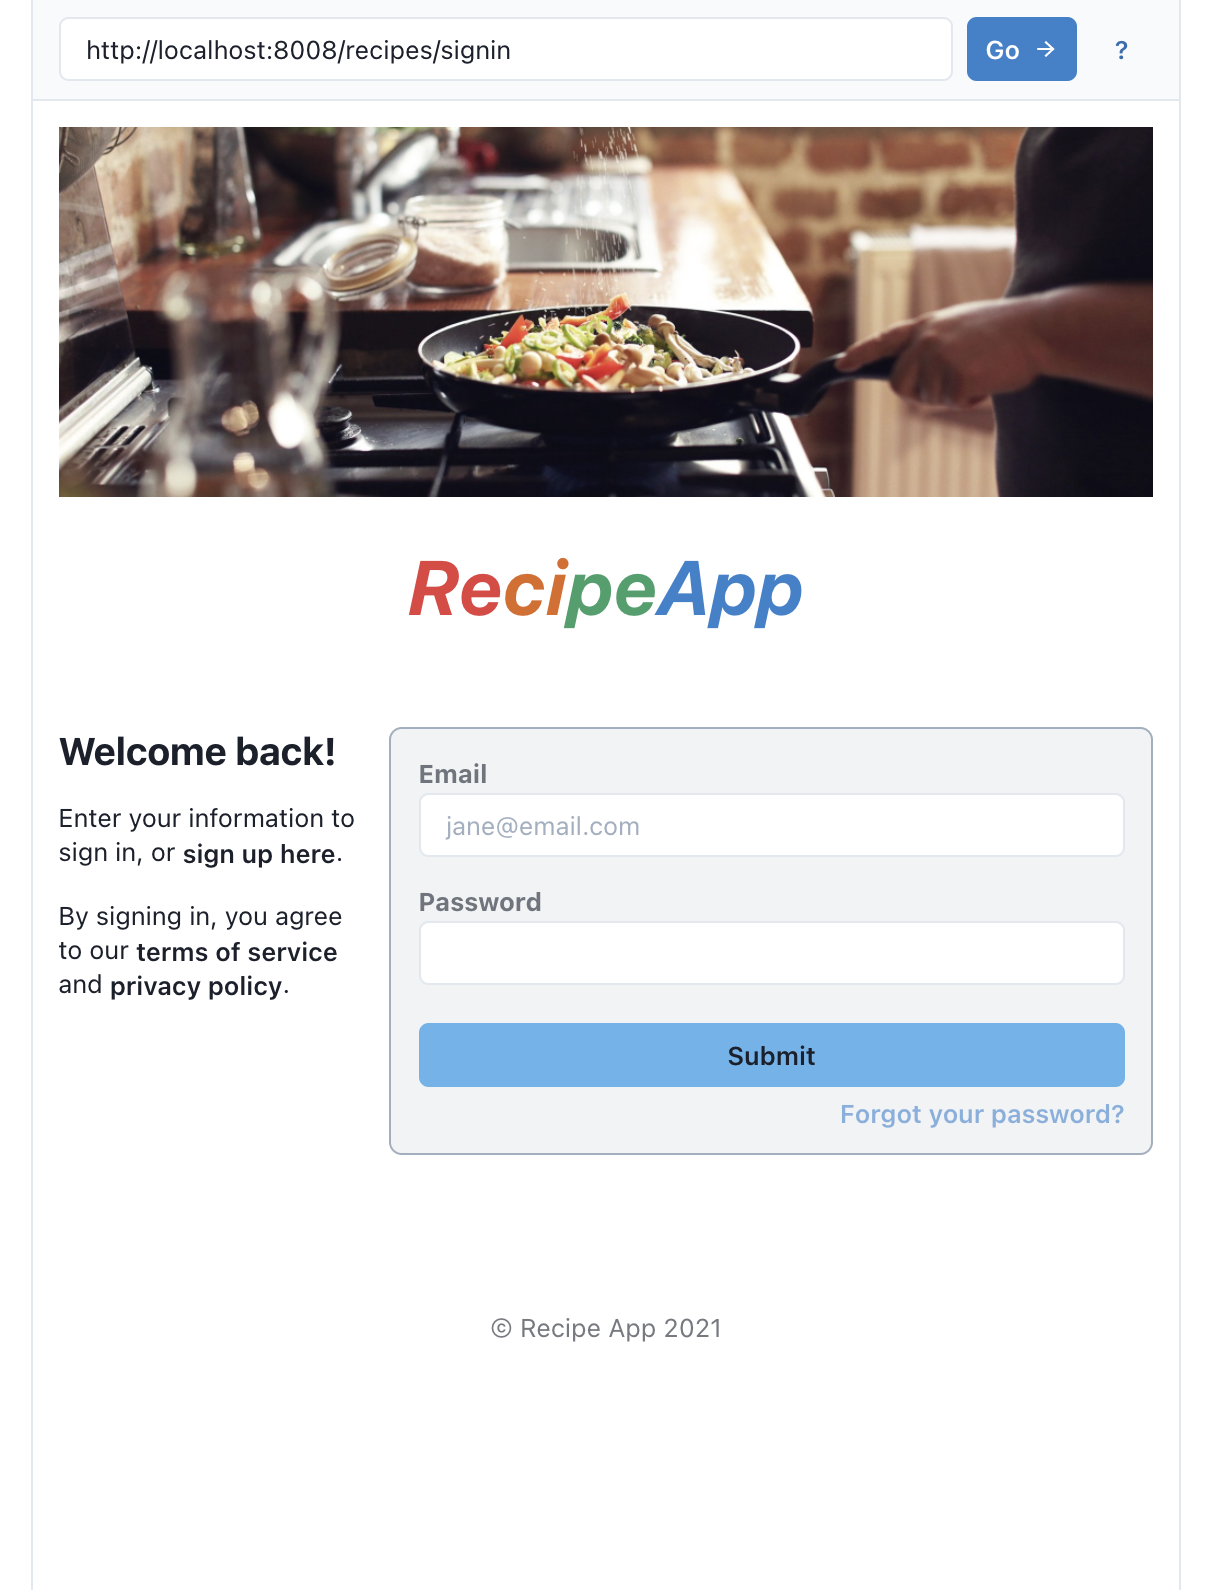
\includegraphics[width=6.2cm]{thesis/paper/images/rec_signin.png}
  \,
  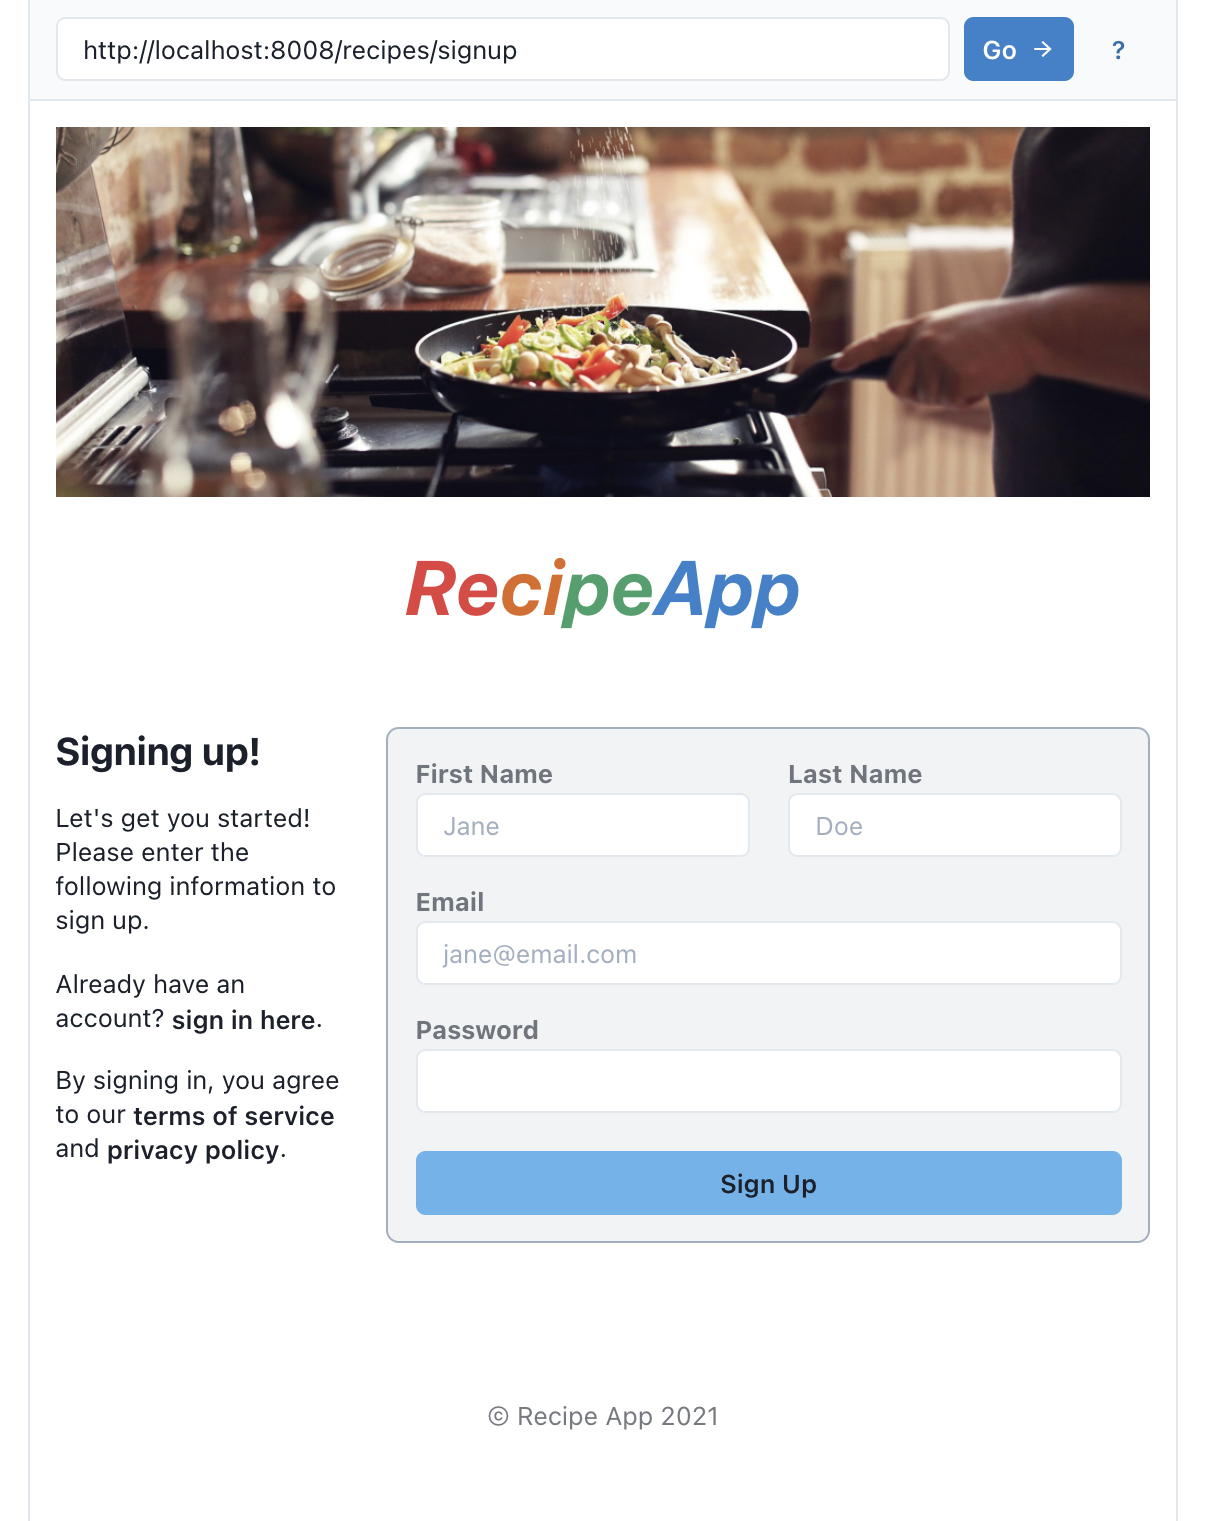
\includegraphics[width=6.2cm]{thesis/paper/images/res_signup.png}
  \caption{RecipeApp Sign In/Sign Up screens}%
  \label{fig:rec_signin_signup}%
\end{figure}

First, user visits the URL the RecipeApp is served from via the address bar above. In figure \ref{fig:rec_signin_signup} the example server runs on \texttt{http://localhost:3000} and the endpoint RecipeApp is served from is \texttt{/recipes}. If user is not already signed in, they will be redirected to \texttt{/recipes/signin}. After signing in from this screen, they will be redirected back to the application. If they were visiting a particular URL such as \texttt{/recipes/new} or \texttt{/recipes/3} before they got redirected to the sign in screen, they will be redirected back to that screen after signing in. Once they are signed in, they will be presented with the recipe list. Recipe list has two view options, grid view and list view, which user can chose between. The view selection will persist across sessions. Moreover, the list features a search bar, which can be used to search recipes by keywords. On each recipe item, there difficulty and time it takes to prepare the recipe is displayed along with an image. From the top navigation, user can click on the Add Recipe button to go to the insert page. From there, they can insert their own recipe.

\subsection{Authentication}

Before the authentication, first thing to understand is how we implemented the redirection system. The redirect screen, which can be seen in figure \ref{fig:rec_redirect}, is essentially an handlebars template that can be rendered with some parameters and can be used for different purposes. There are two essential functions of this screen; it instructs Intertext client to store some data, and to redirect user to another endpoint. The parameters changes based on the user case.

\begin{figure}[htb]
  \centering
  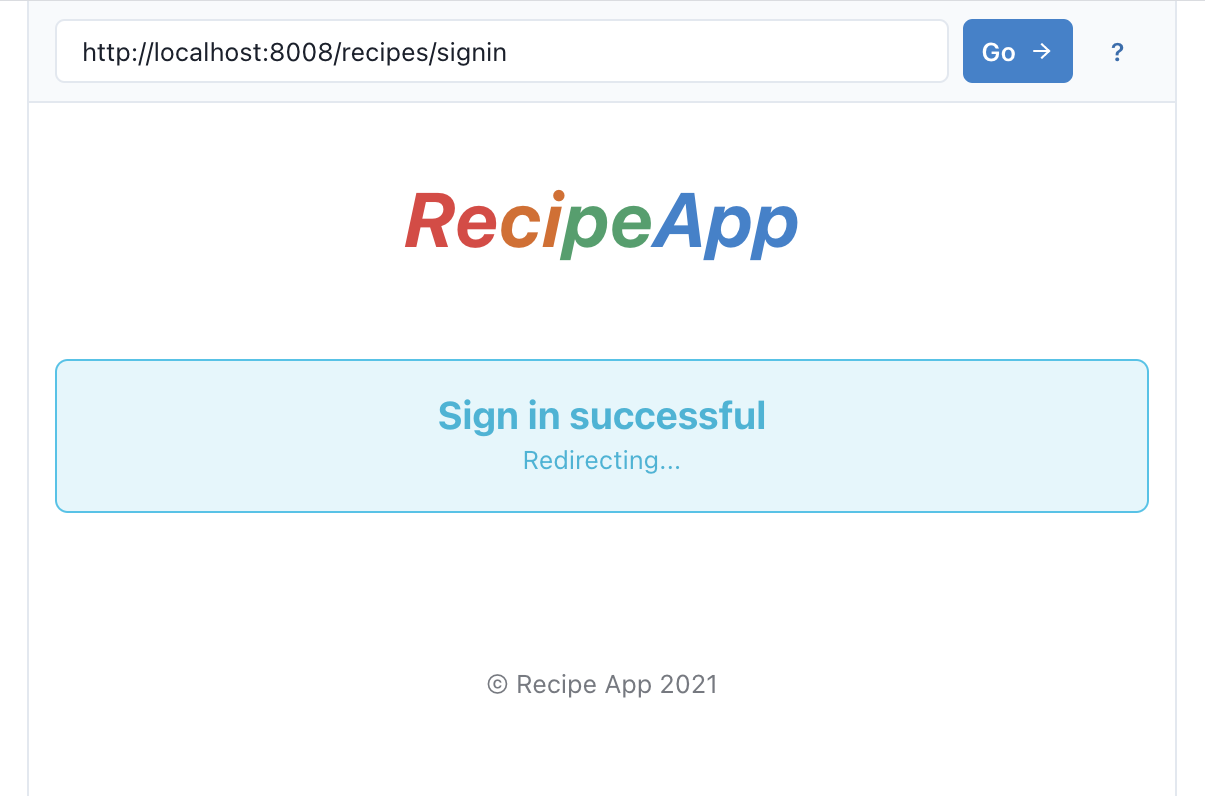
\includegraphics[width=12.4cm]{thesis/paper/images/rec_redirect.png}
  \caption{Redirect screen}%
  \label{fig:rec_redirect}%
\end{figure}

As we established before, Intertext clients passes on the application state along with every single request. When user visits the application URL, the server receives the persisted state, which is where the user token is expected to be if the user is logged in. When a user lands on any page of RecipeApp that is behind the authentication wall, the server checks the presence of \texttt{token} in request body, and if it is not present, it renders the redirect screen as shown in figure \nameref{fig:token_capture}. 

\begin{figure}[htb]
\begin{minipage}{\linewidth}
\begin{lstlisting}[language=javascript]
const token = get(req, "body.persist.token");
if (!token) {
  res.render(view("redirect"), { ... });
} else {
  res.render(view("home"), { ... });
}
\end{lstlisting}
\end{minipage}
\caption{How token is captured on the backend}%
\label{fig:token_capture}%
\end{figure}

The redirect screen does two things: it instructs the client to store a variable called \texttt{auth-callback} which holds the URL that user is at, and it instructs the Intertext client to navigate to the \texttt{/signin} endpoint. Intertext clients does these two things, and redirects user to the \texttt{/signin} endpoint, triggering another request to the backend. The \texttt{/signin} endpoint on the backend renders the sign in form. After user submits the form with their credentials, another request to the \texttt{/signin} endpoint is made, but this time with the credentials. Backend then checks the credentials, and if it is a successful login, it once again renders the redirect screen. The redirect screen again performs two tasks: first it instructs the Intertext client to store the \texttt{token} to the persisted storage. Then, if the \texttt{auth-callback} variable is present in the request body of the request made to the \texttt{/signin} endpoint (which is where the URL user was redirected to the sign in endpoint from is stored at), it instructs the Intertext client to redirect back to that endpoint, otherwise it redirects to the home screen.

\subsection{Recipe List}

The recipes view features a list of the recipes. As seen in in figure \ref{fig:rec_recipe_list}, it has several components: recipe title, description, difficulty and time to cook details that are displayed in tags, and a read more button to navigate to the recipe page. The difficulty tags are made of the \texttt{block} component, and they use intents to hint the difficulty of the recipe. The view has two display options, a list view and a grid view. It also has a search input to search recipes.

\begin{figure}[htb]
  \centering
  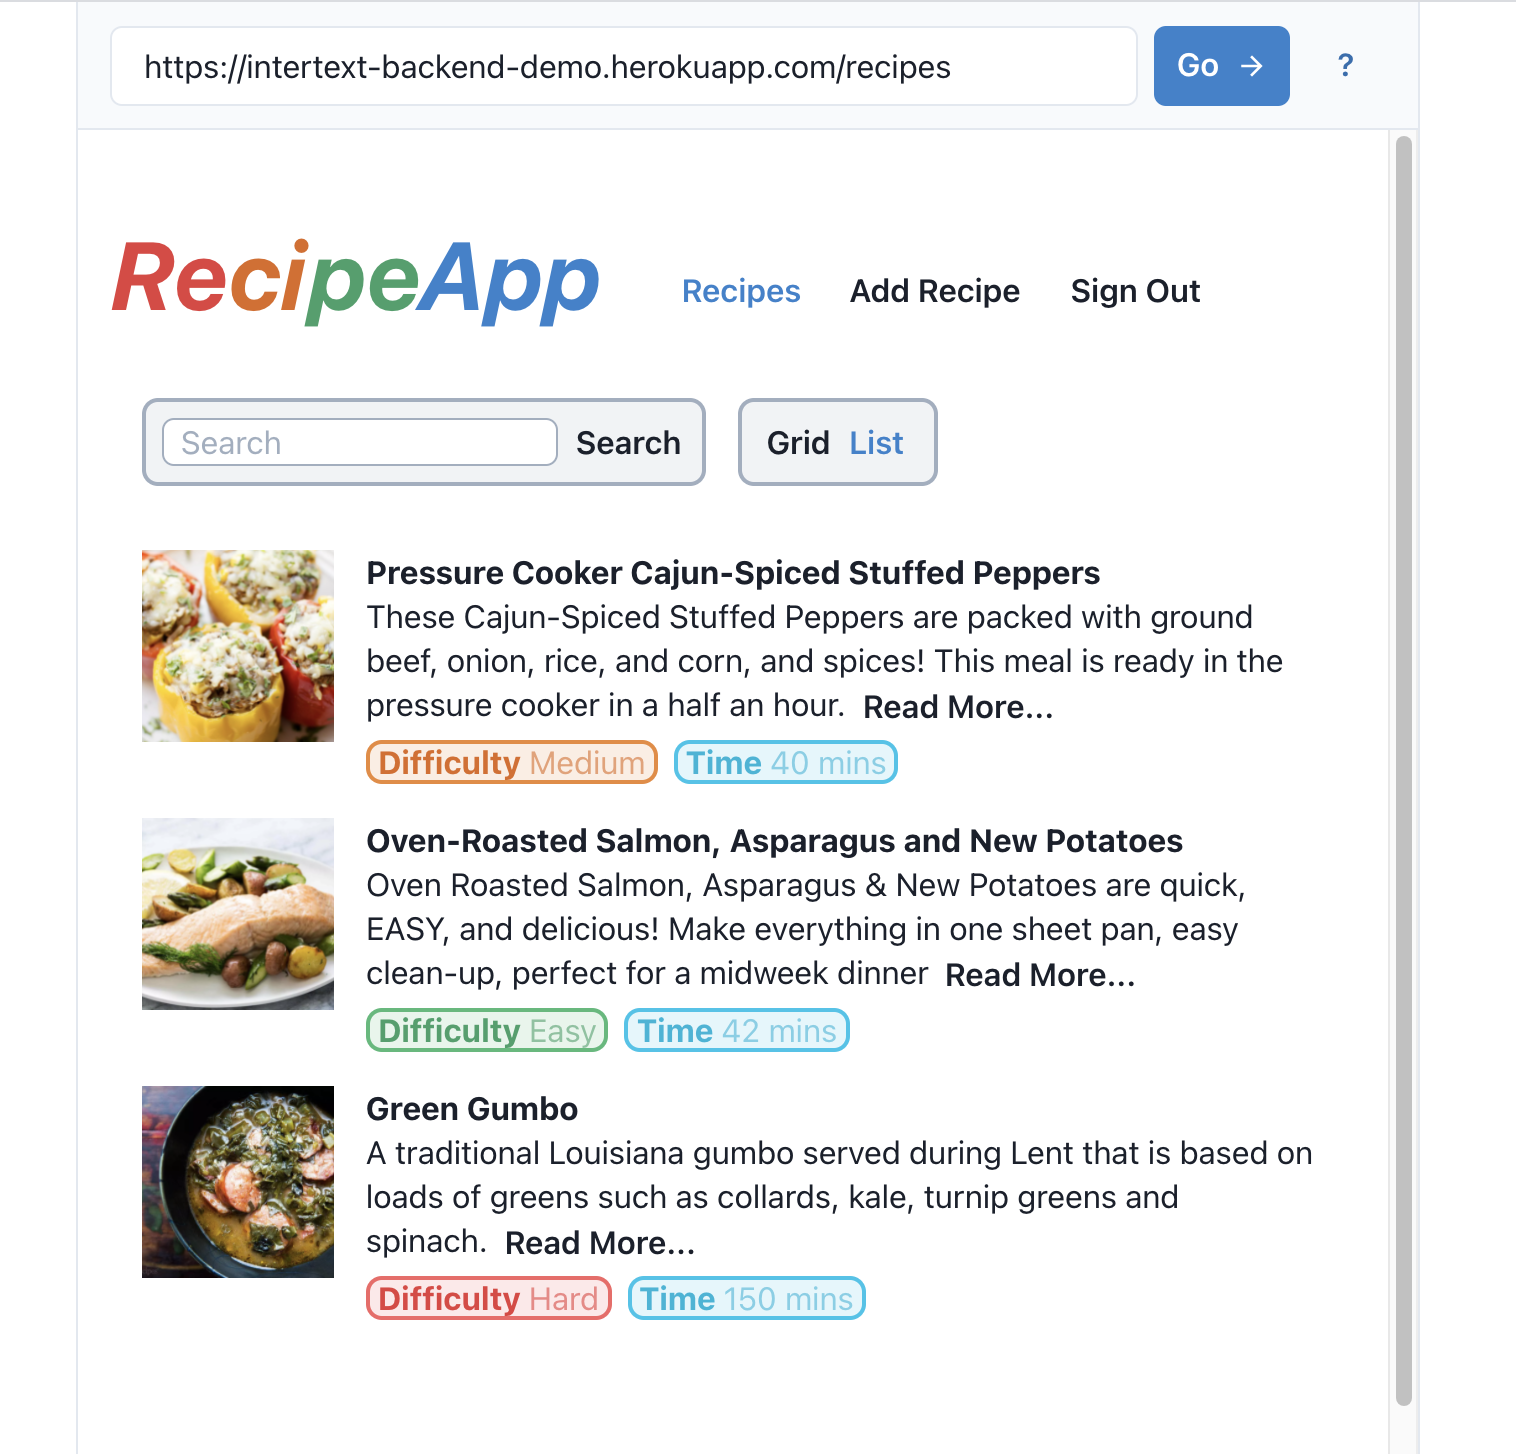
\includegraphics[width=6.2cm]{thesis/paper/images/recipe_list.png}
  \,
  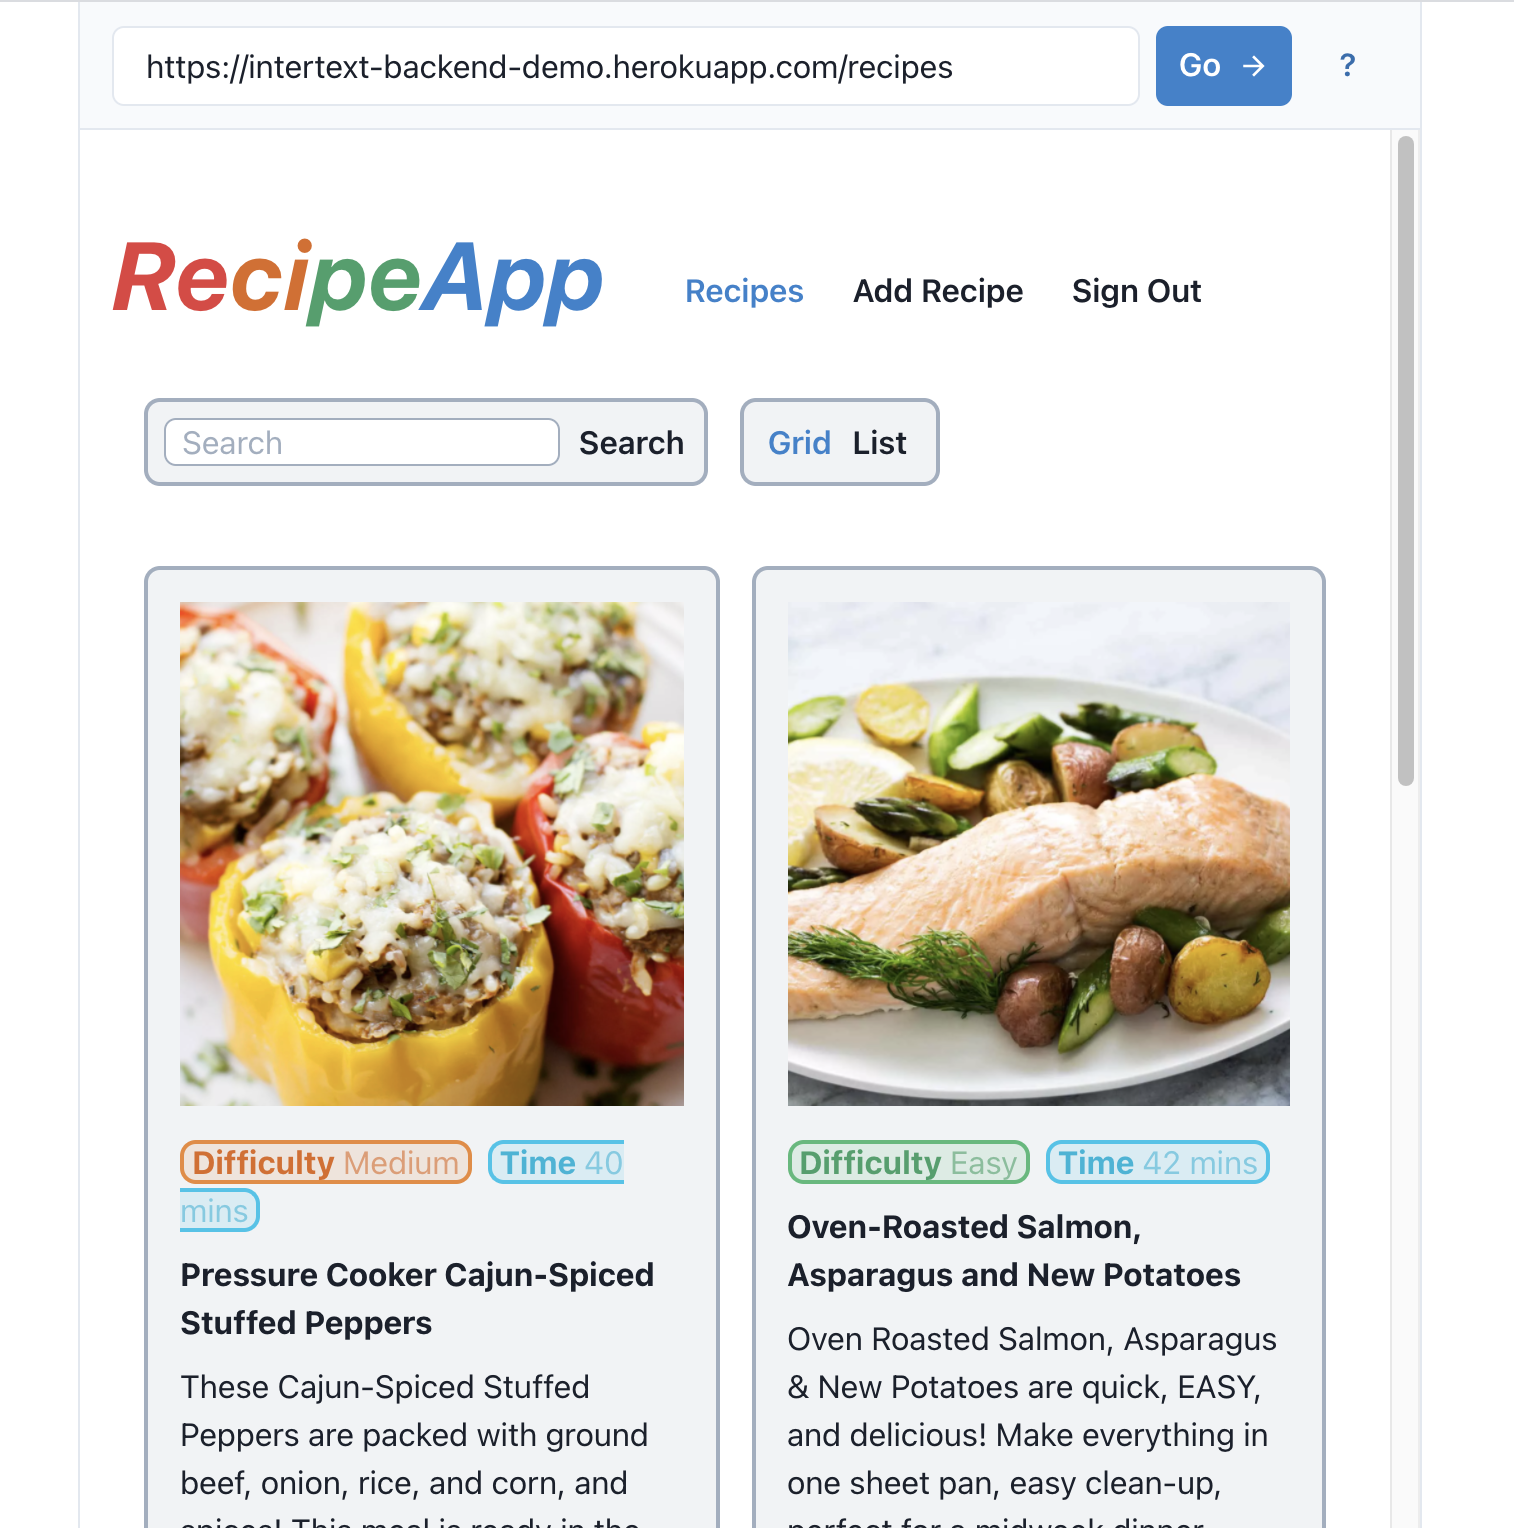
\includegraphics[width=6.2cm]{thesis/paper/images/recipe_grid.png}
  \caption{RecipeApp Recipe List Grid/List Views}%
  \label{fig:rec_recipe_list}%
\end{figure}

Both the input and display preference options work in the same way, by modifying the front-end state and triggering a request to the backend to pick up the modified state. As user types into the text input, Intertext client automatically saves its value into the state that gets passed on to the backend on every request. The "Search" button next to the search input only triggers a request to the \texttt{/recipes} endpoint. The recipes endpoint receives the query in the search input, and filters the results accordingly. It also pre-populates the input value by passing the query as a children to the \texttt{input} component. The display options on the other hand first sets the front-end state variable \texttt{layout} to either \texttt{grid} or \texttt{list}, and again triggers a request to the same \texttt{recipes} endpoint as seen in figure \ref{fig:rec_display_options}. The backend picks up the variable and renders the different version of the displays accordingly. The primary color of the button for the active display option is also controlled by the same \texttt{layout} variable, backend renders the buttons with the relevant intent based on that variable also as seen in figure \ref{fig:rec_display_options}.

\begin{figure}[htb]
\begin{minipage}{\linewidth}
\begin{lstlisting}[language=xml]
{{#> button_small}}
  <text intent="{{#if layout_grid}}primary{{else}}{{/if}}">Grid</text>
  <button.onClick>
    <state key="layout" persist="true">grid</state>
    <request endpoint="/recipes"></request>
  </button.onClick>
{{/button_small}}
{{#> button_small}}
  <text intent="{{#if layout_list}}primary{{else}}{{/if}}">List</text>
  <button.onClick>
    <state key="layout" persist="true">list</state>
    <request endpoint="/recipes"></request>
  </button.onClick>
{{/button_small}}
\end{lstlisting}
\end{minipage}
\caption{Redirect screen example}%
\label{fig:rec_display_options}%
\end{figure}


\section{Evaluation}

In this section, we explain how we conducted our user study for user evaluation. We first explain our methodology, and then share the results of our evaluation.

\subsection{Methodology}

We conducted our user study in the form of surveys. We used Google Forms to create the survey and manage the responses. In the surveys, we first gave some information and/or material to investigate, then followed it with likert scale questions.

We utilised Amazon's Mechanical Turk (MTurk) service in order to find participants. We stated the description and intentions of each survey on their respective survey page. Some of our surveys required special skills, for which we used features provided by MTurk that enables us to only target participants with special skills. We set the compensation price per answer to 10 cents for general participation surveys, and 50 cents for surveys that requires special skills. We required our participants to enter their \textit{worker id} both on the surveys and on the respective survey page on MTurk, so that we can match the responses of the participants with their MTurk profiles to verify only our intended audience has participated, and duplicate/third party responses are eliminated.

Our user evaluation was conducted in two stages. First stage was to validate the problems in our problem statement that we are intending to solve, and the second stage was to validate Intertext, the solution we offer in order to address these problems. 

\paragraph{Phase 1: Problem Validation}

Here we aimed to validate the problem we are intending to solve. We first asked some optional identifying questions to ask about the background of the participants; including their age, gender, country of origin and occupation. Then, we separated questions into groups for every main category in our \nameref{problemStatement} section. We directed this section only towards the end-users.

\paragraph{Phase 2: Solution Validation}

Our project targets two different user group; developers, and end-users. Developers will use Intertext technology to develop products and services, and their end-users will use applications made within the Intertext platform. Both developers and end-users have separate benefits. In this phase of the user evaluation, we targeted both developers and end-users. 

We created two separate surveys, one for developers and one for end-users. On the survey we prepared for the end-users, we first gave a brief explanation of what Intertext is and what it does without going into technical details. We told about Intertext clients, how it works and how it can be used. We kept it as simple as possible, to make sure the general public can understand it. We also linked to a demo from the Intertext web client. Then, similarly to what we did in the first phase, we stated every problem from the \nameref{problemStatement} section. For every problem, we wrote a short paragraph explaining what the problem exactly is, and one explaining how Intertext addresses that problem. Then, we followed it with likert scale questions. 

For the developer survey, we started it off by duplicating the one for end-users and removing the questions. We kept the information parts identical, as developers also needs to understand what Intertext does and why it is beneficial to the users. We then created an extra section to give a technical overview of how Intertext works, benefits, and how Intertext applications can be developed. We also included a link to the repository that hosts \texttt{RecipeApp}, our demo Intertext application. Next, we listed the developer-related problems from the \nameref{problemStatement} section, wrote a paragraph explaining it, and another paragraph explaining the solution. We followed it with likert scale questions just like in end-user survey format.

In our likert scale questions, we focused on the trade-offs in order to get answers as objective as possible. To elaborate on this, if we were to explained that we solved a problem, and then followed it with a question asking about the thoughts on the solution, the responses would most certainly be positive. Solving a problem often comes with a trade-off, and this trade-off might not be immediately visible to the participant. We attempted to ask questions in a way that raises an awareness about the trade-offs, and validates if participant is on board with the solution regardless of it. For example, one of the solutions we offer is guaranteed security by eliminating third-party code execution, and the trade-off of this is that the platform will not support rich front-end functionalities and experiences. For general public, this trade-off would likely be overlooked. Thus, the likert scale question we asked about this solution was \textit{I would prefer guaranteed privacy and security over rich front-end functionality}, validating that users care more about privacy and security than rich front-end functionality.

\subsection{Phase 1 Results}

In the first phase, we received 119 responses (after filtering out duplicate answers and answers with invalid worker ids). Our results for the first phase are very positive, we were able to validate the problem and implement Intertext with more confidence. First three graphs shows age distribution, gender and country of origin of the respondents, and the ones that follows shows the responses given to each question alongside the question text underneath.

\begin{figure}[H]
  \centering
  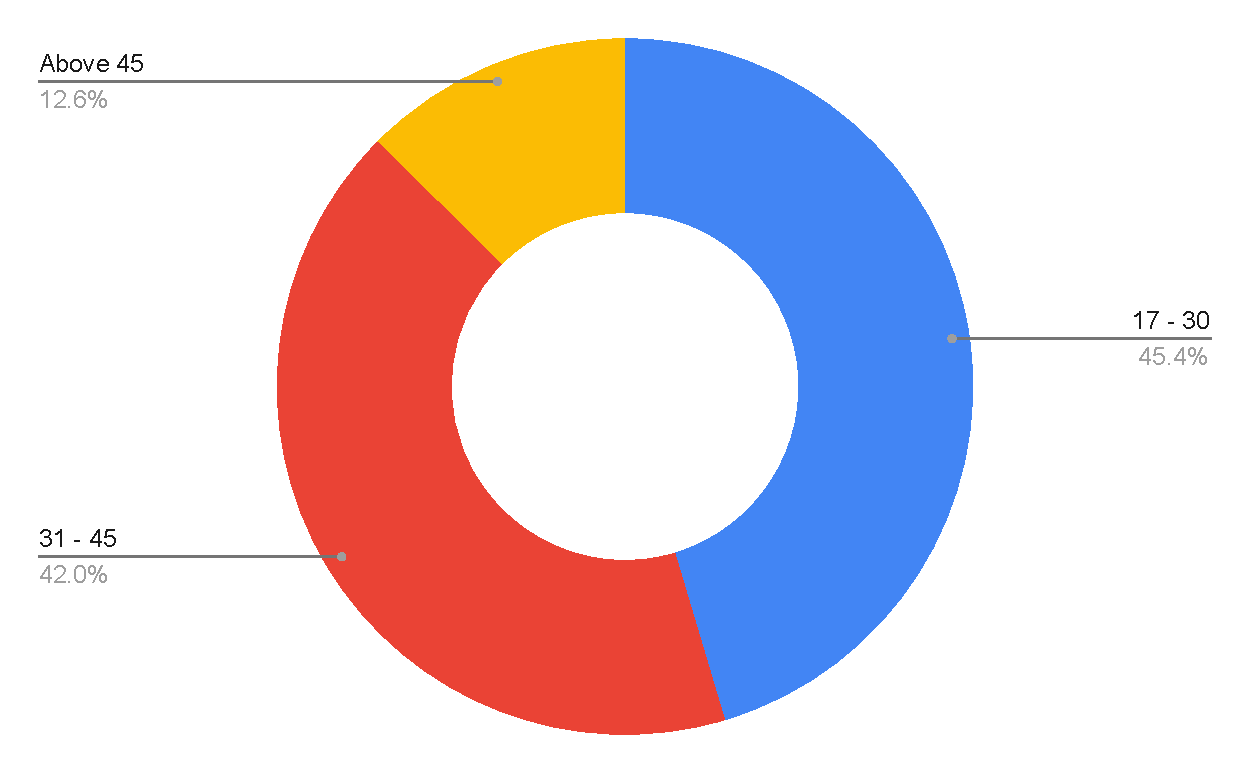
\includegraphics[width=13cm]{thesis/paper/images/p1_age.pdf}
  \textbf{Age distribution}
\end{figure}

\begin{figure}[H]
  \centering
  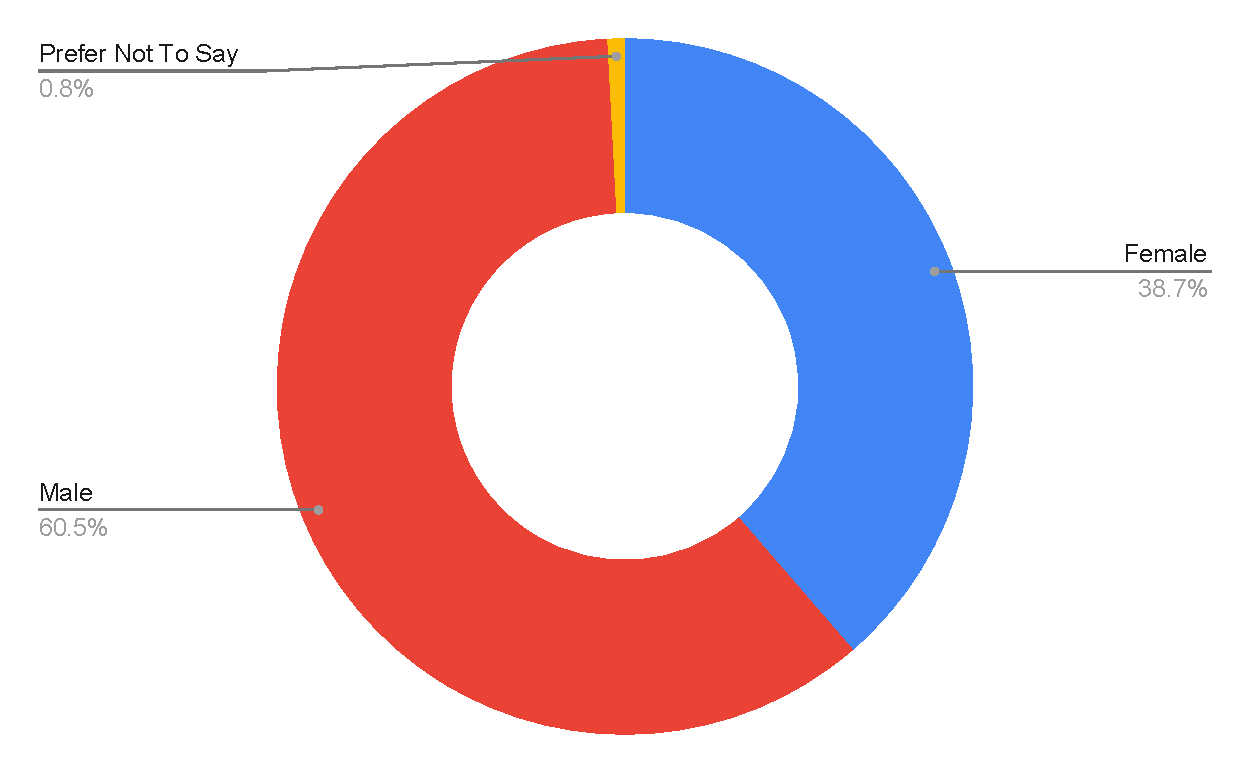
\includegraphics[width=13cm]{thesis/paper/images/p1_gender.pdf}
  \textbf{Gender distribution}
\end{figure}

\begin{figure}[H]
  \centering
  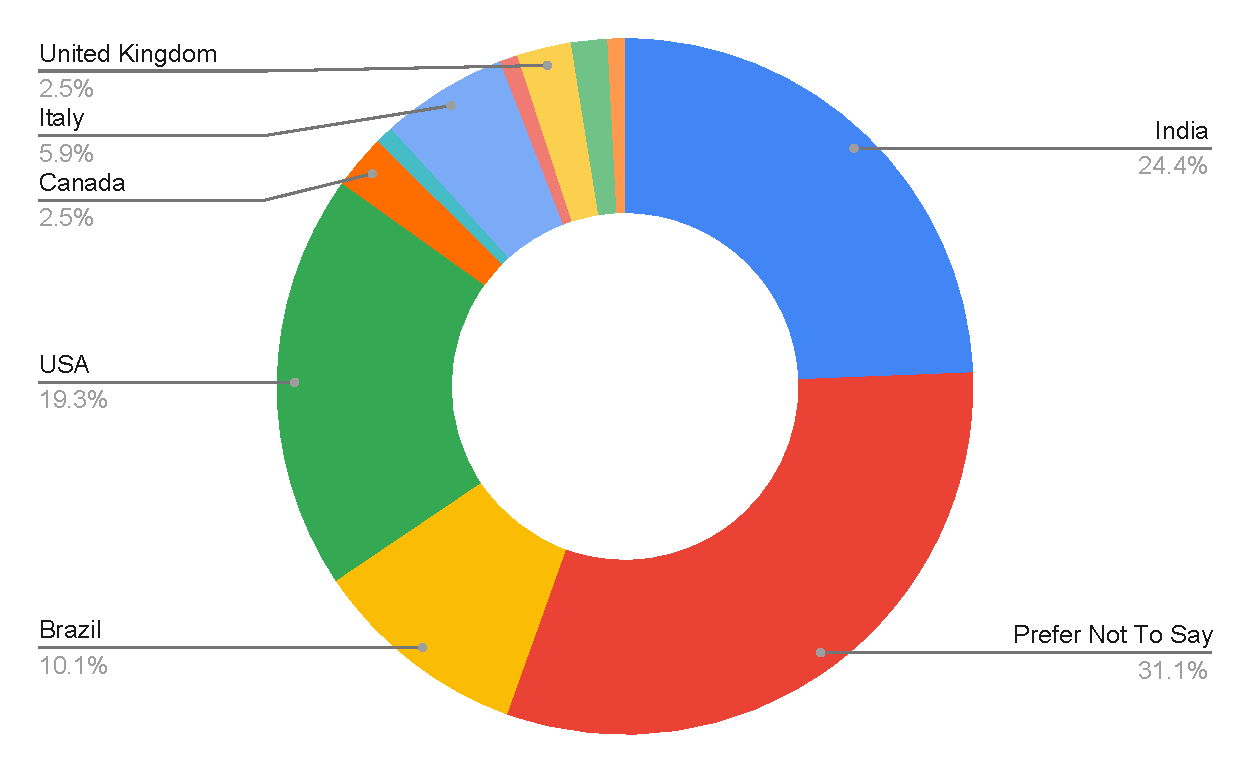
\includegraphics[width=13cm]{thesis/paper/images/p1_country.pdf}
  \textbf{Country of Origin}
\end{figure}

\begin{figure}[H]
  \centering
  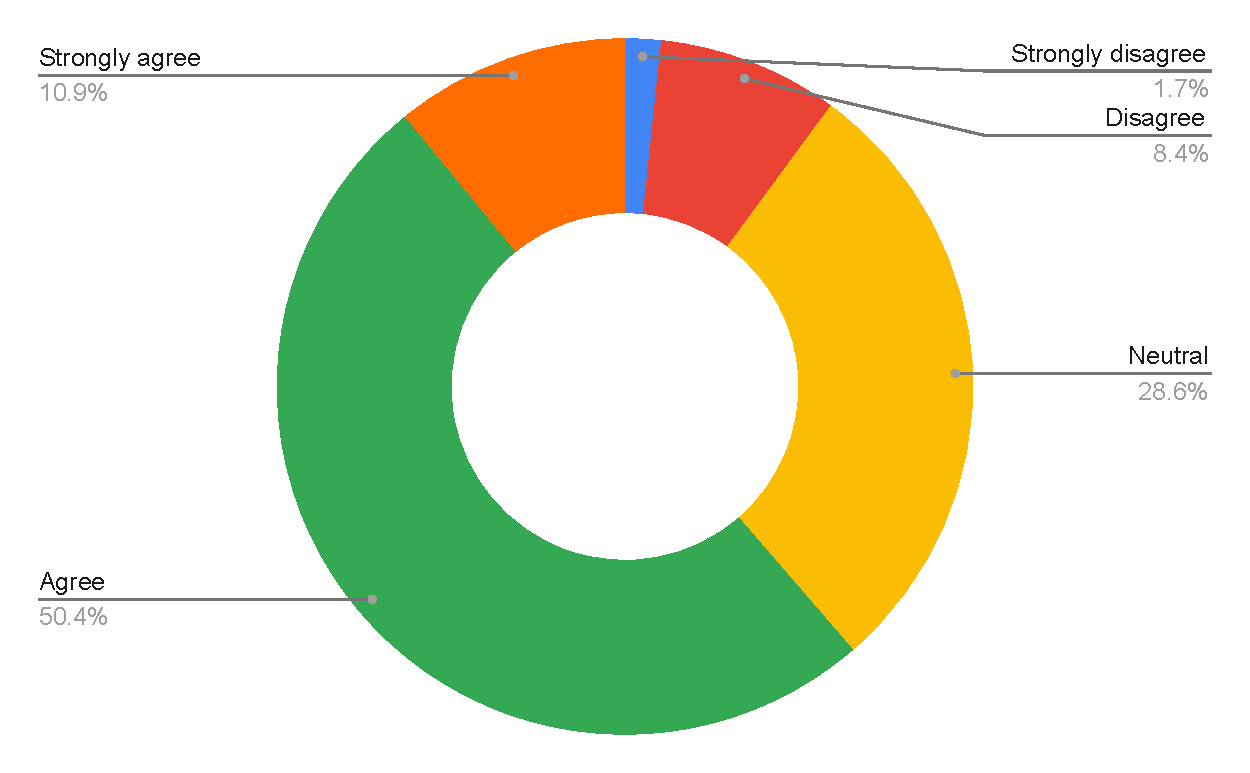
\includegraphics[width=13cm]{thesis/paper/images/p1_q1.pdf}
  \textbf{Question:} I experience UI/UX inconsistencies in some applications
\end{figure}

\begin{figure}[H]
  \centering
  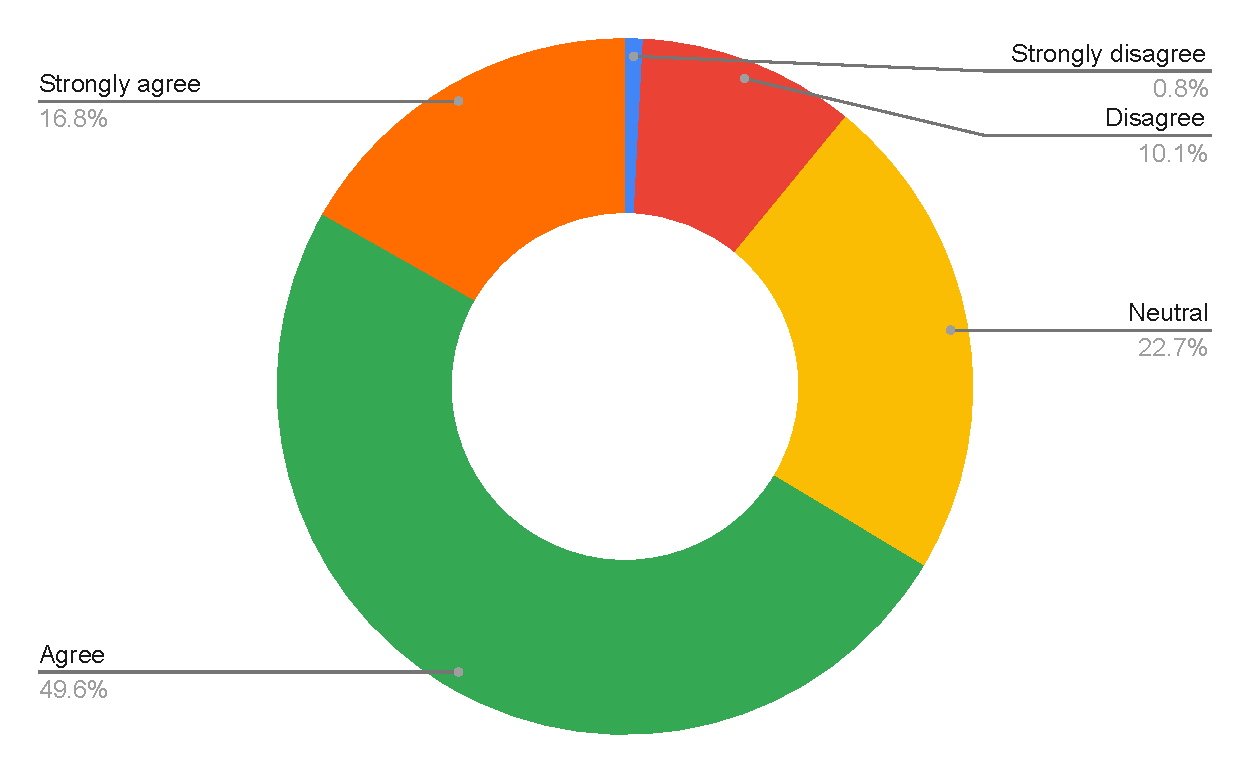
\includegraphics[width=13cm]{thesis/paper/images/p1_q2.pdf}
  \textbf{Question:} I sometimes experience poor design in some applications
\end{figure}

\begin{figure}[H]
  \centering
  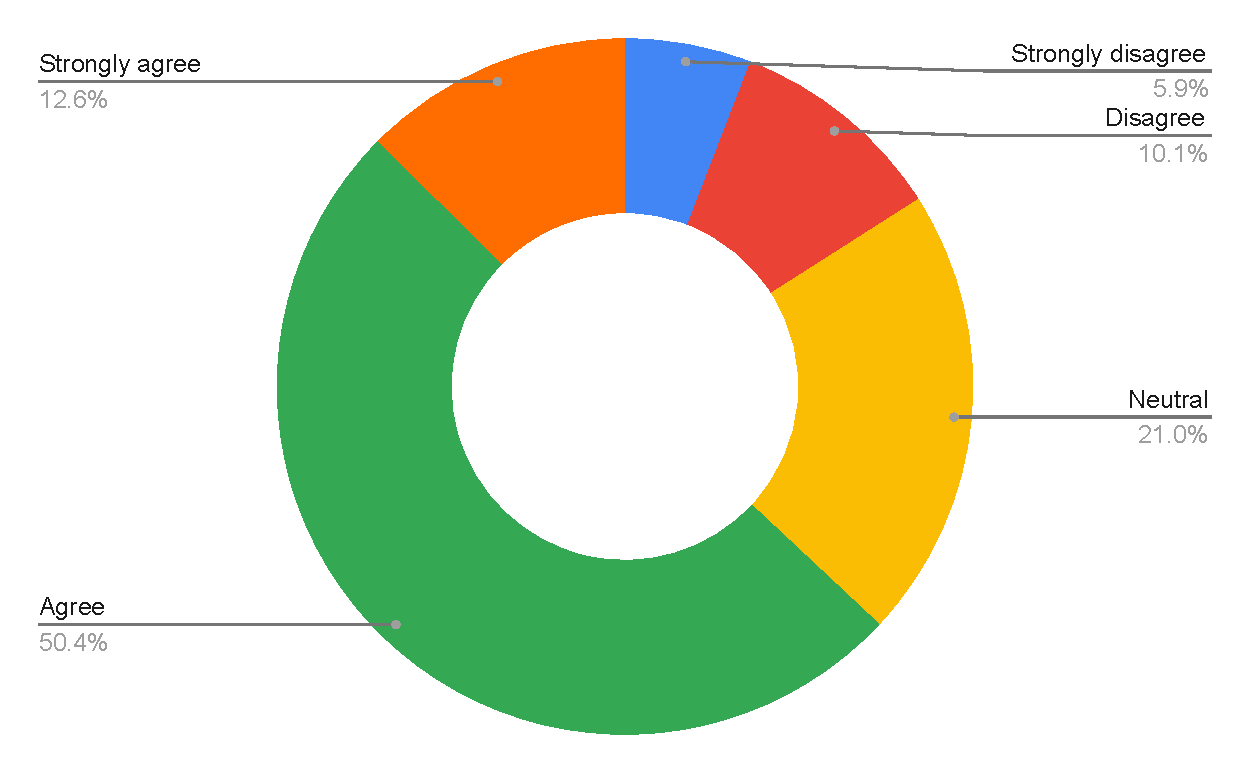
\includegraphics[width=13cm]{thesis/paper/images/p1_q3.pdf}
  \textbf{Question:} Advertisement sector is out of control
\end{figure}

\begin{figure}[H]
  \centering
  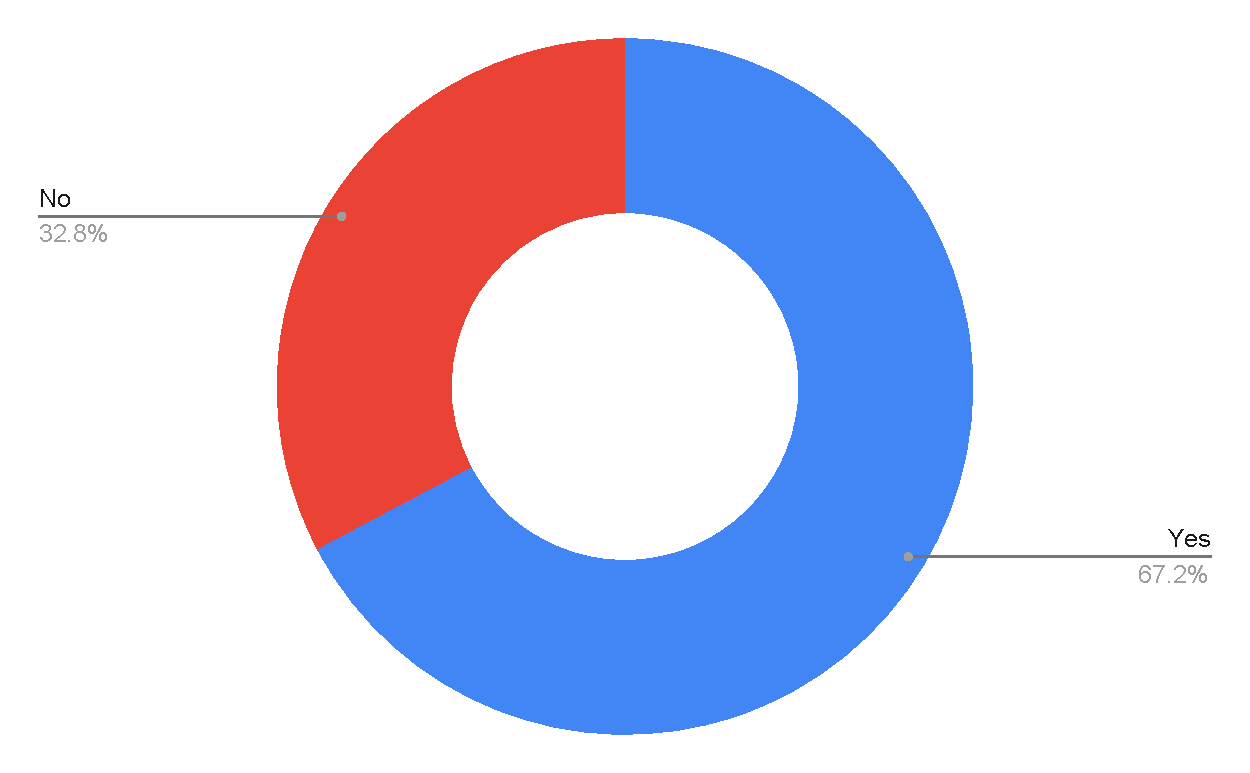
\includegraphics[width=13cm]{thesis/paper/images/p1_q4.pdf}
  \textbf{Question:} I use an AdBlocker
\end{figure}

\begin{figure}[H]
  \centering
  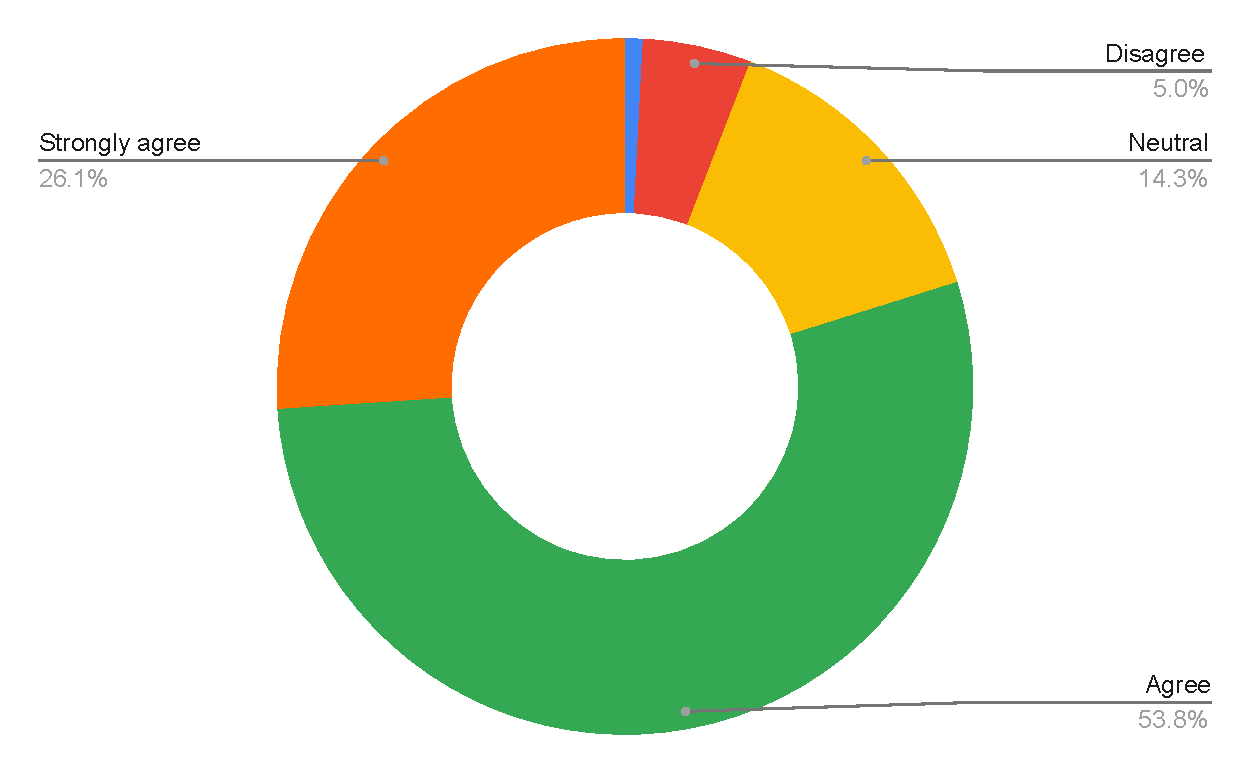
\includegraphics[width=13cm]{thesis/paper/images/p1_q5.pdf}
  \textbf{Question:} I'm often frustrated with ads on the internet
\end{figure}

\begin{figure}[H]
  \centering
  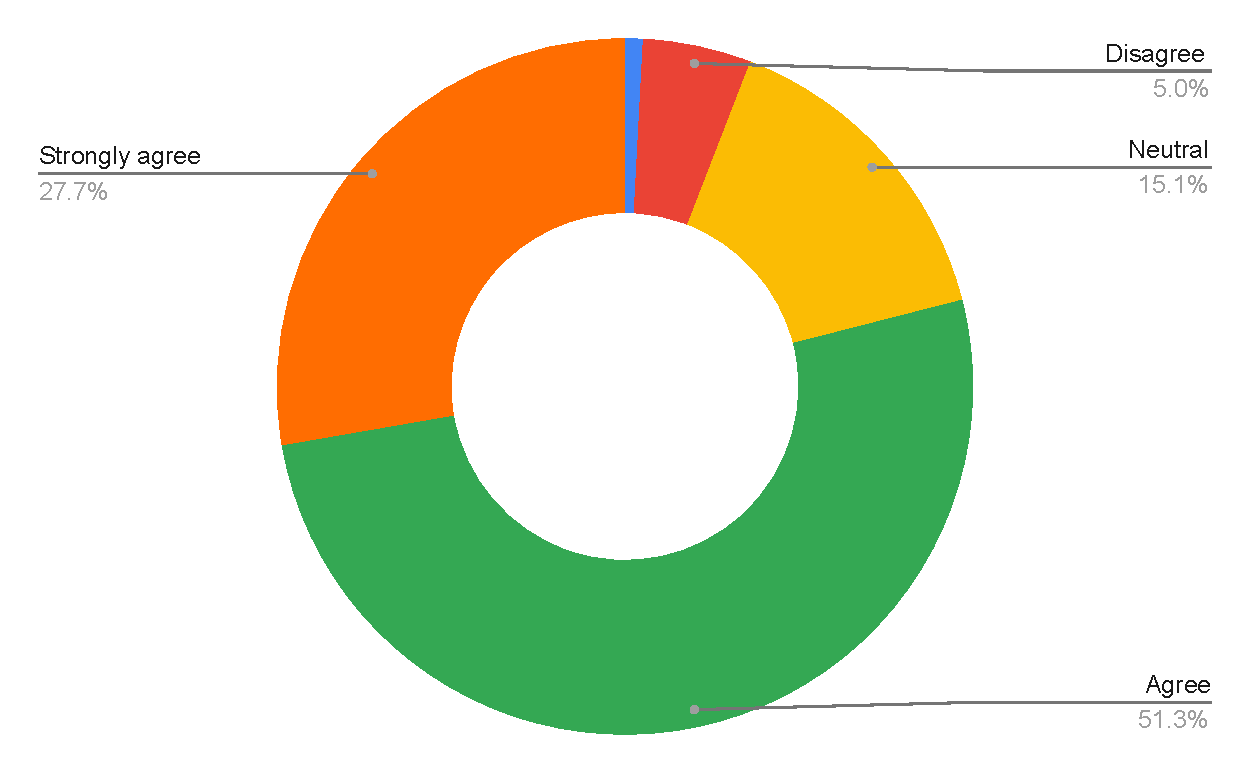
\includegraphics[width=13cm]{thesis/paper/images/p1_q6.pdf}
  \textbf{Question:} I'm often frustrated with ads on mobile/desktop apps
\end{figure}

\begin{figure}[H]
  \centering
  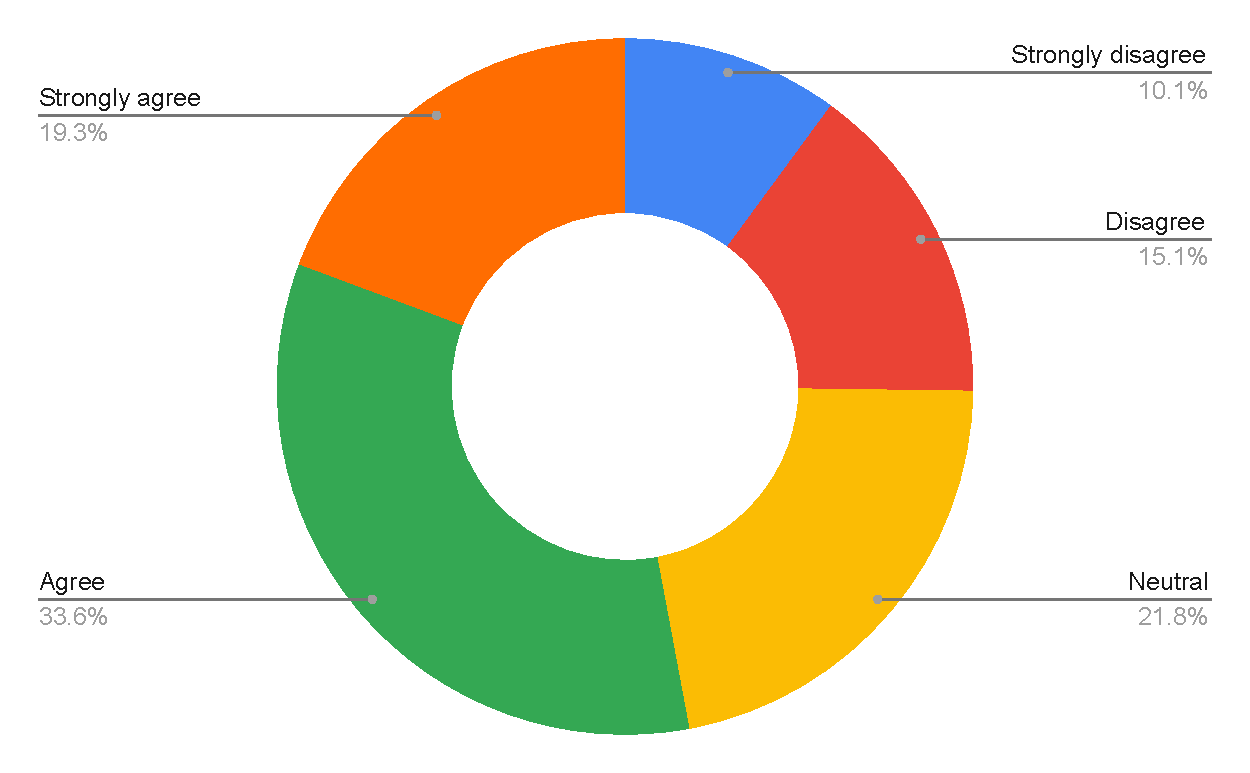
\includegraphics[width=13cm]{thesis/paper/images/p1_q7.pdf}
  \textbf{Question:} I would rather pay a small fee than seeing ads
\end{figure}

\begin{figure}[H]
  \centering
  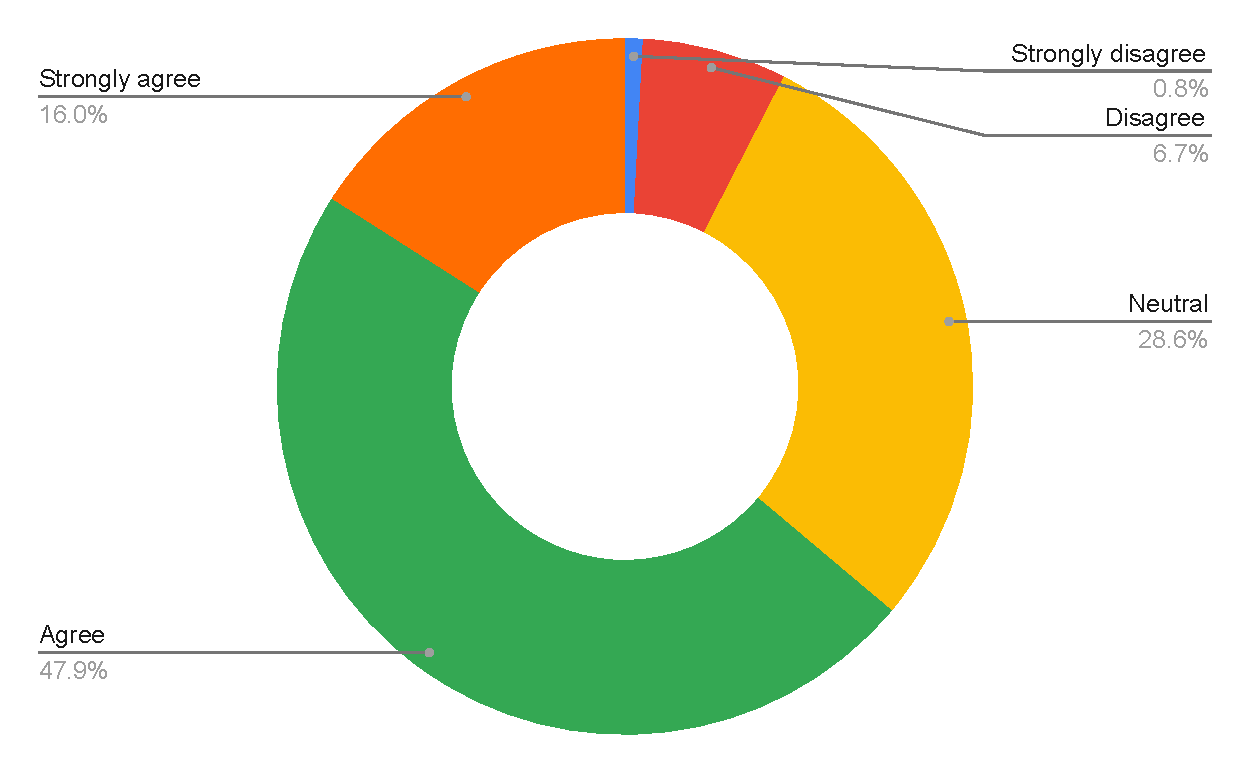
\includegraphics[width=13cm]{thesis/paper/images/p1_q8.pdf}
  \textbf{Question:} I wish I was able to customise the appearances of websites/applications.
\end{figure}

\begin{figure}[H]
  \centering
  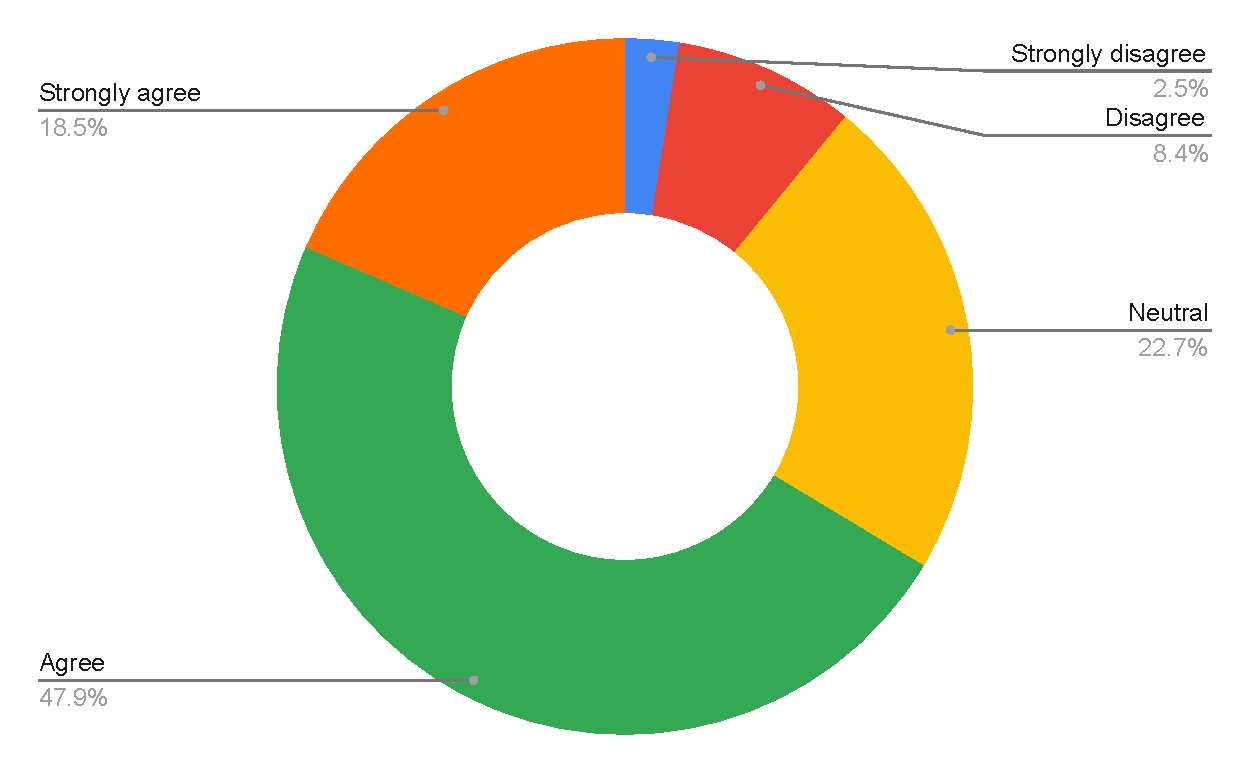
\includegraphics[width=13cm]{thesis/paper/images/p1_q9.pdf}
  \textbf{Question:} I wish I could choose or create a universal theme that would apply to all websites/applications
\end{figure}

\begin{figure}[H]
  \centering
  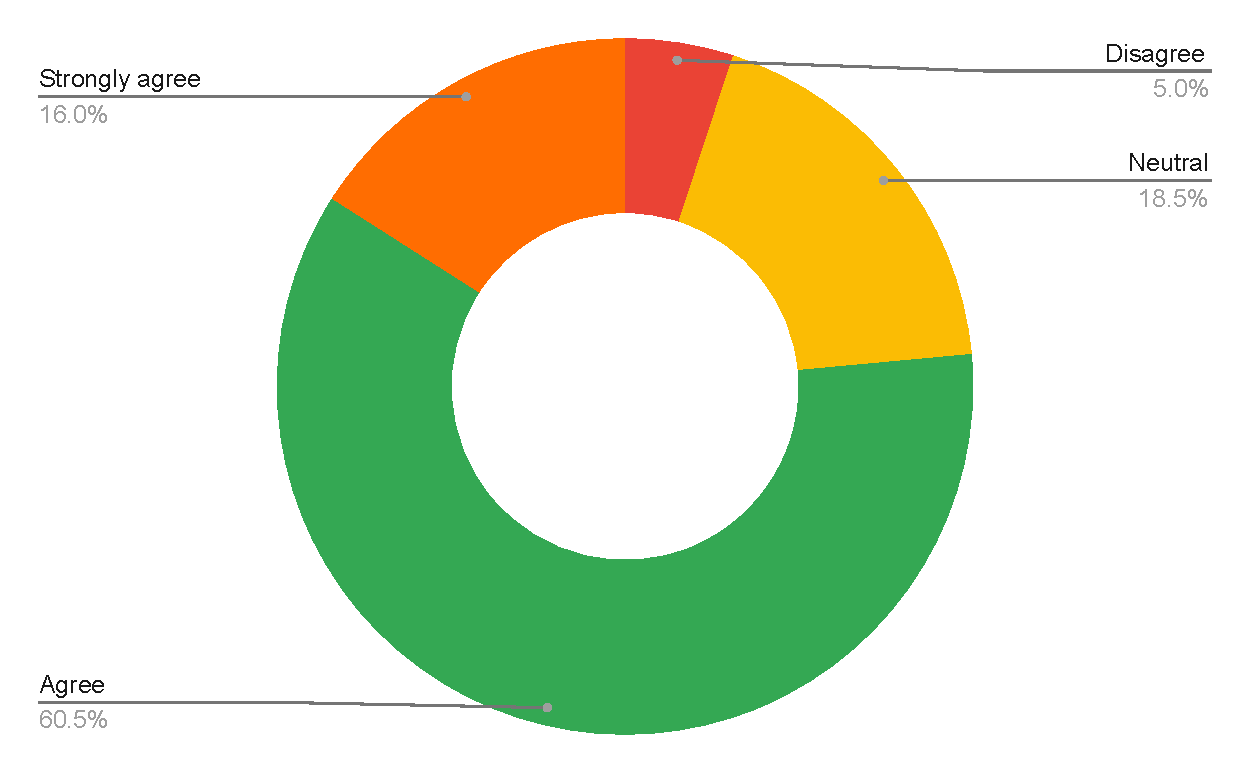
\includegraphics[width=13cm]{thesis/paper/images/p1_q10.pdf}
  \textbf{Question:} Applications I use on a daily basis are mostly available on all my devices/platforms
\end{figure}

\begin{figure}[H]
  \centering
  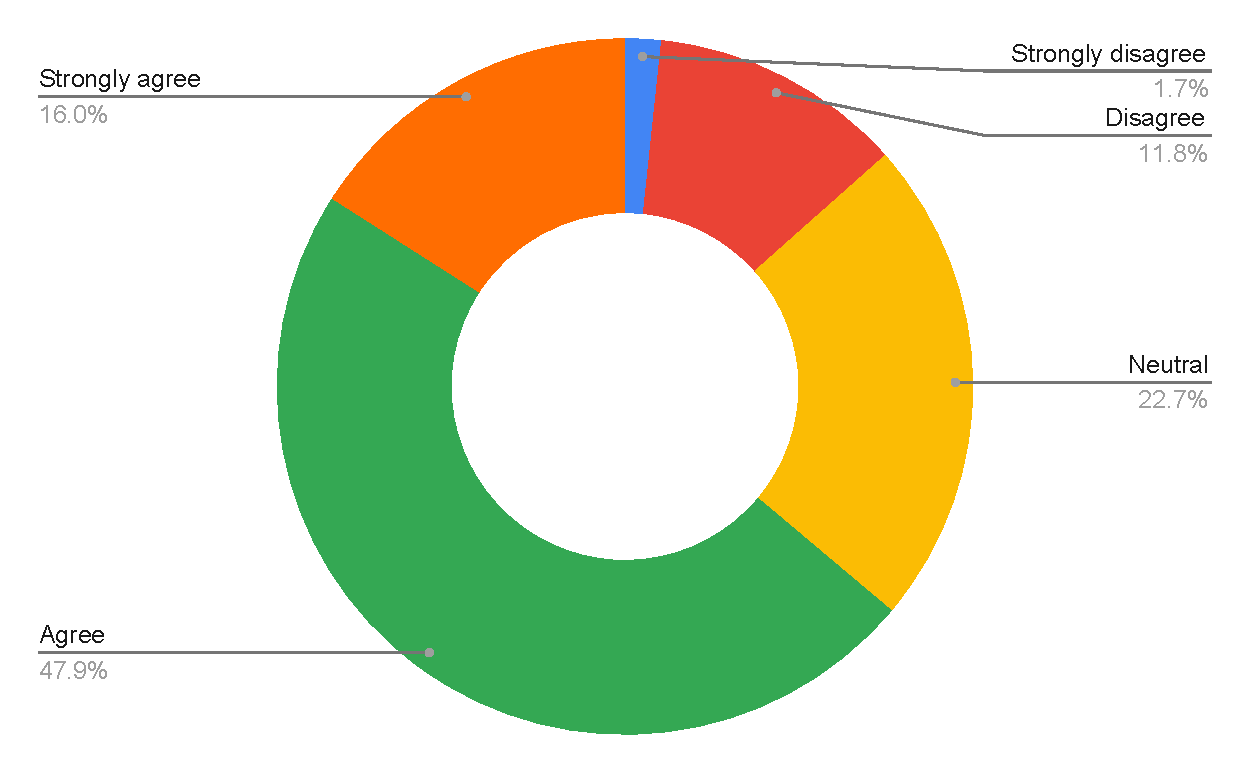
\includegraphics[width=13cm]{thesis/paper/images/p1_q11.pdf}
  \textbf{Question:} Occasionally I have to use desktop applications that are not optimised for small screens/touch interfaces on my phone
\end{figure}

\begin{figure}[H]
  \centering
  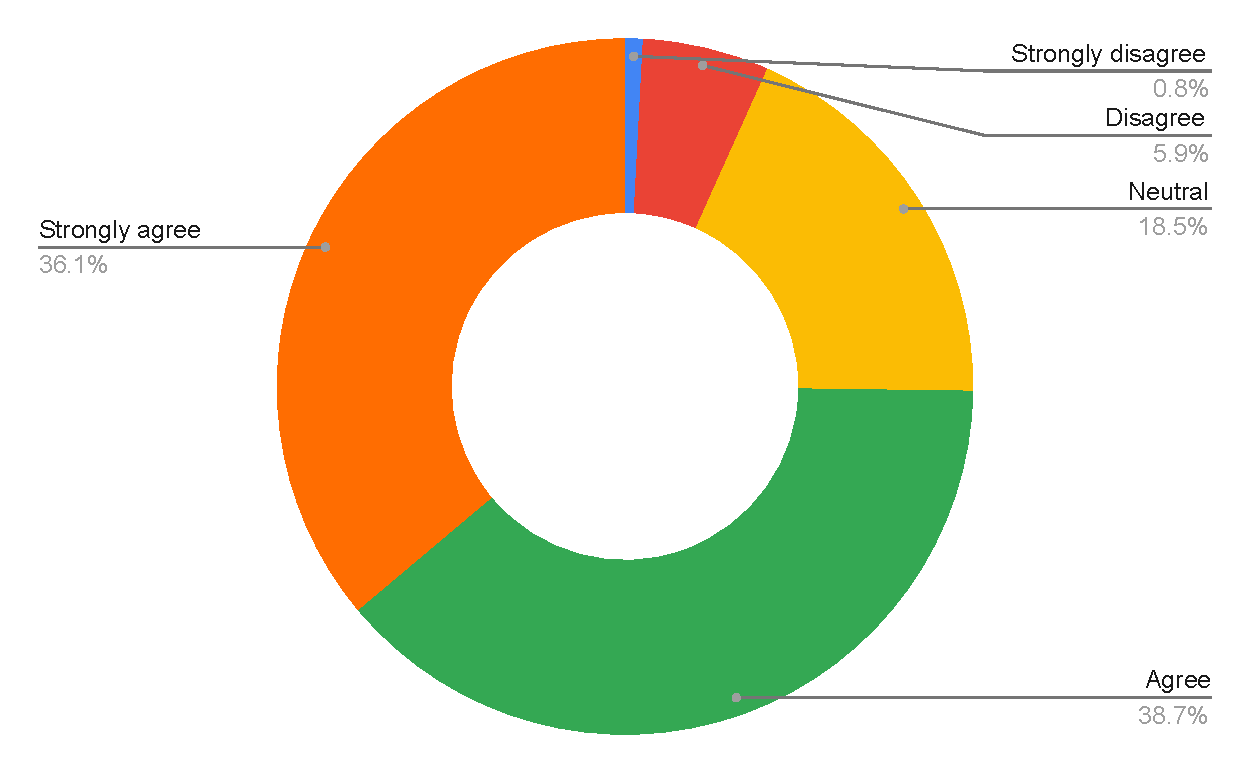
\includegraphics[width=13cm]{thesis/paper/images/p1_q12.pdf}
  \textbf{Question:} If I'm going to use a service just for once, I prefer using their website instead of downloading their application on my phone
\end{figure}

\begin{figure}[H]
  \centering
  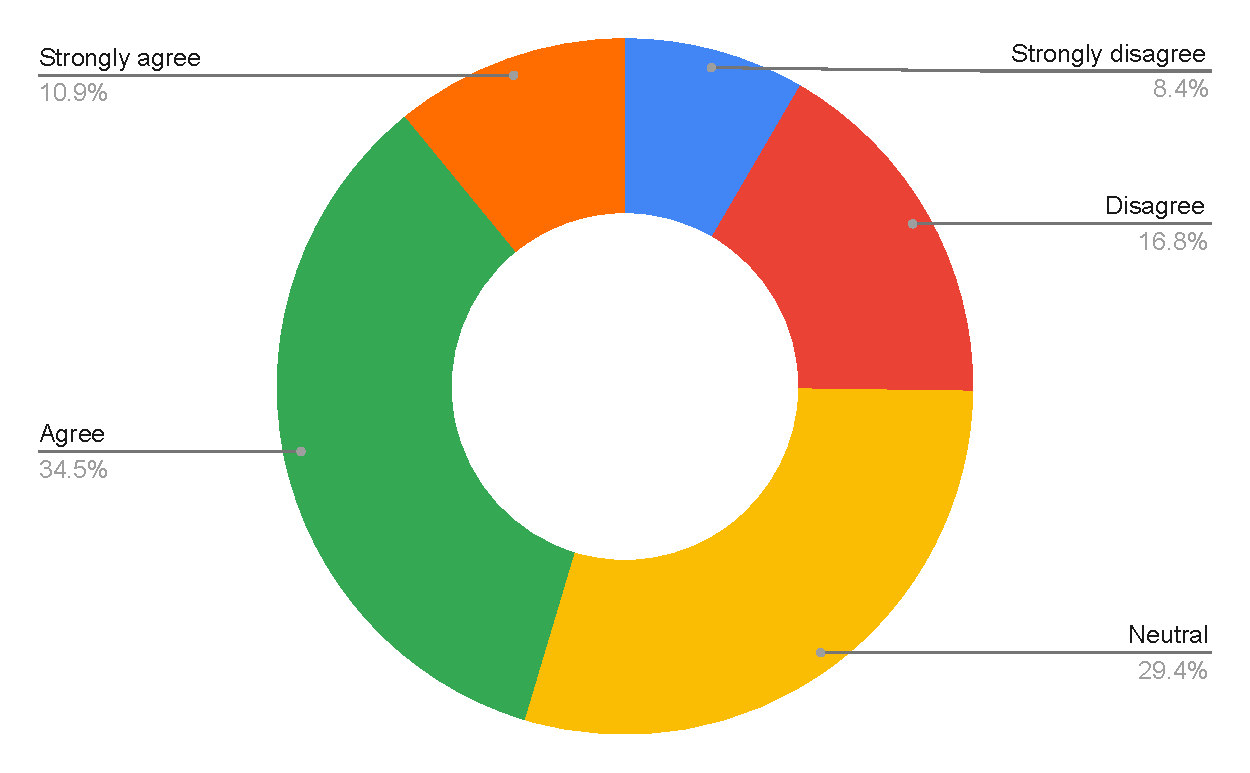
\includegraphics[width=13cm]{thesis/paper/images/p1_q13.pdf}
  \textbf{Question:} I feel safe on the internet
\end{figure}

\begin{figure}[H]
  \centering
  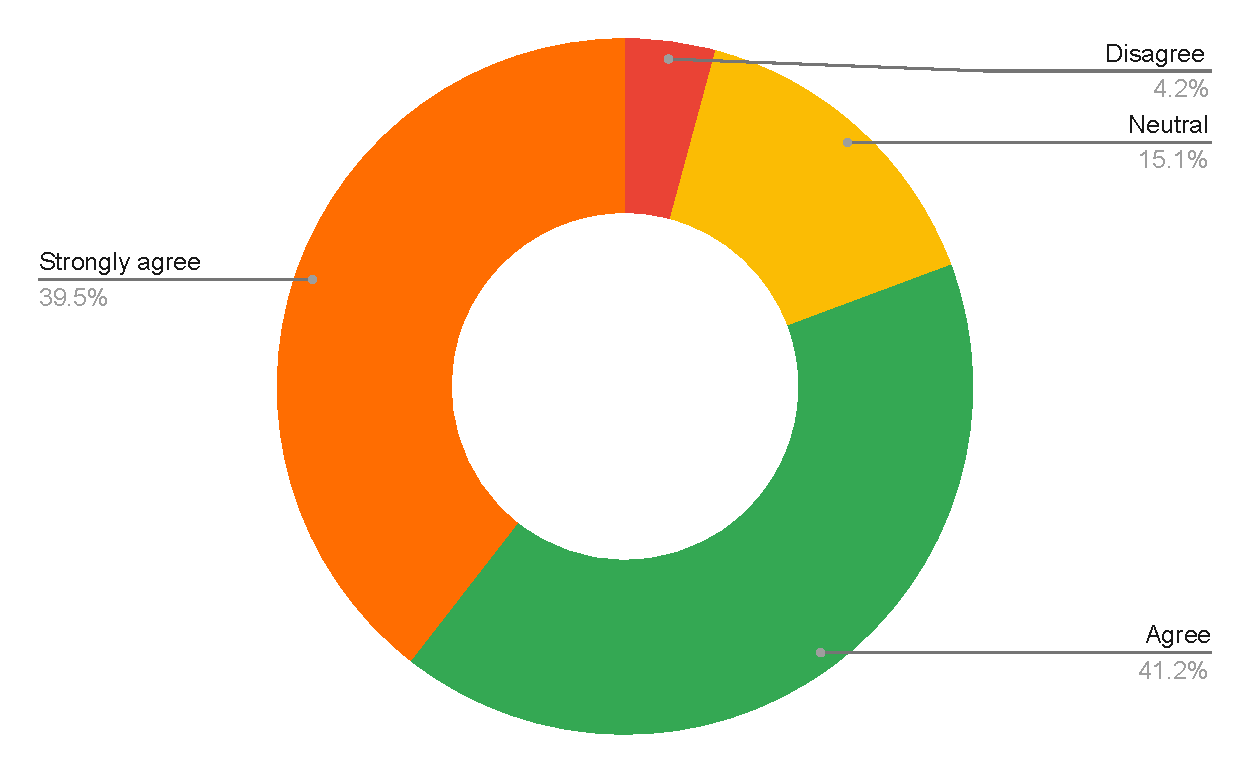
\includegraphics[width=13cm]{thesis/paper/images/p1_q14.pdf}
  \textbf{Question:} I care about my privacy on the internet
\end{figure}

\begin{figure}[H]
  \centering
  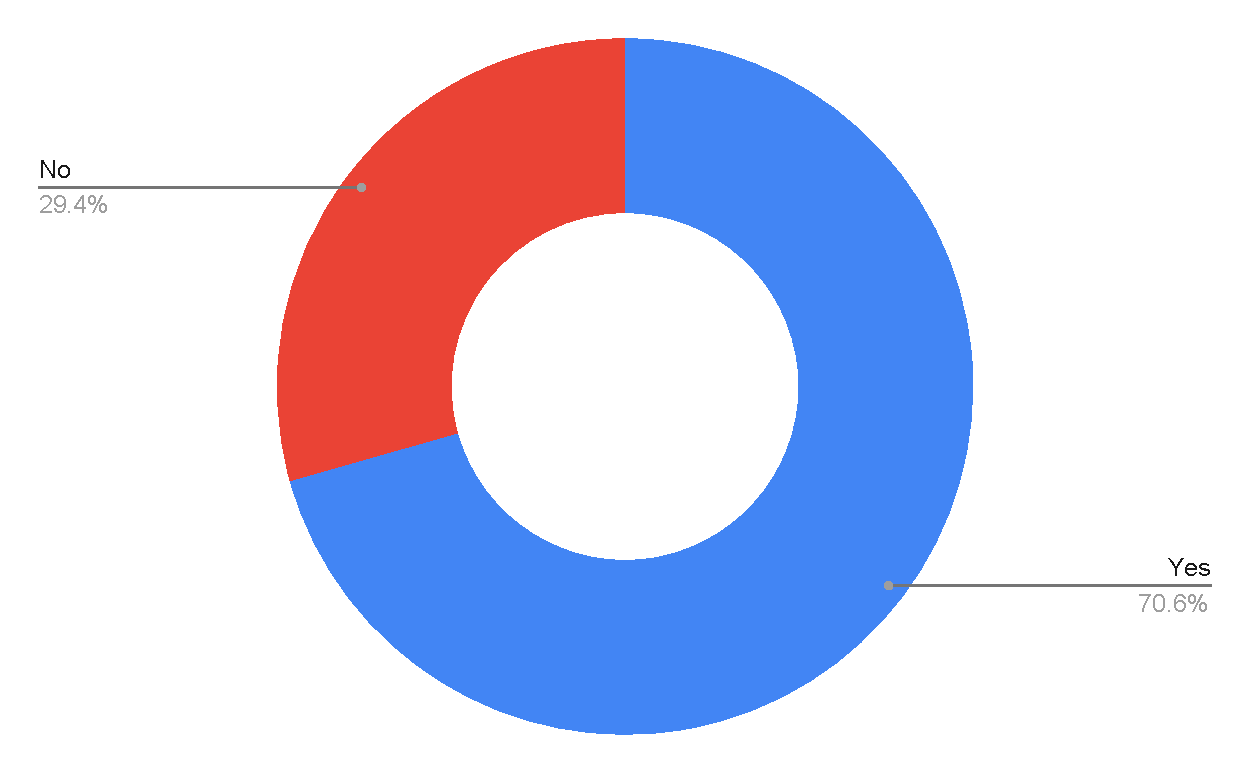
\includegraphics[width=13cm]{thesis/paper/images/p1_q15.pdf}
  \textbf{Question:} Me, or someone I know was targeted by malicious software before
\end{figure}

\begin{figure}[H]
  \centering
  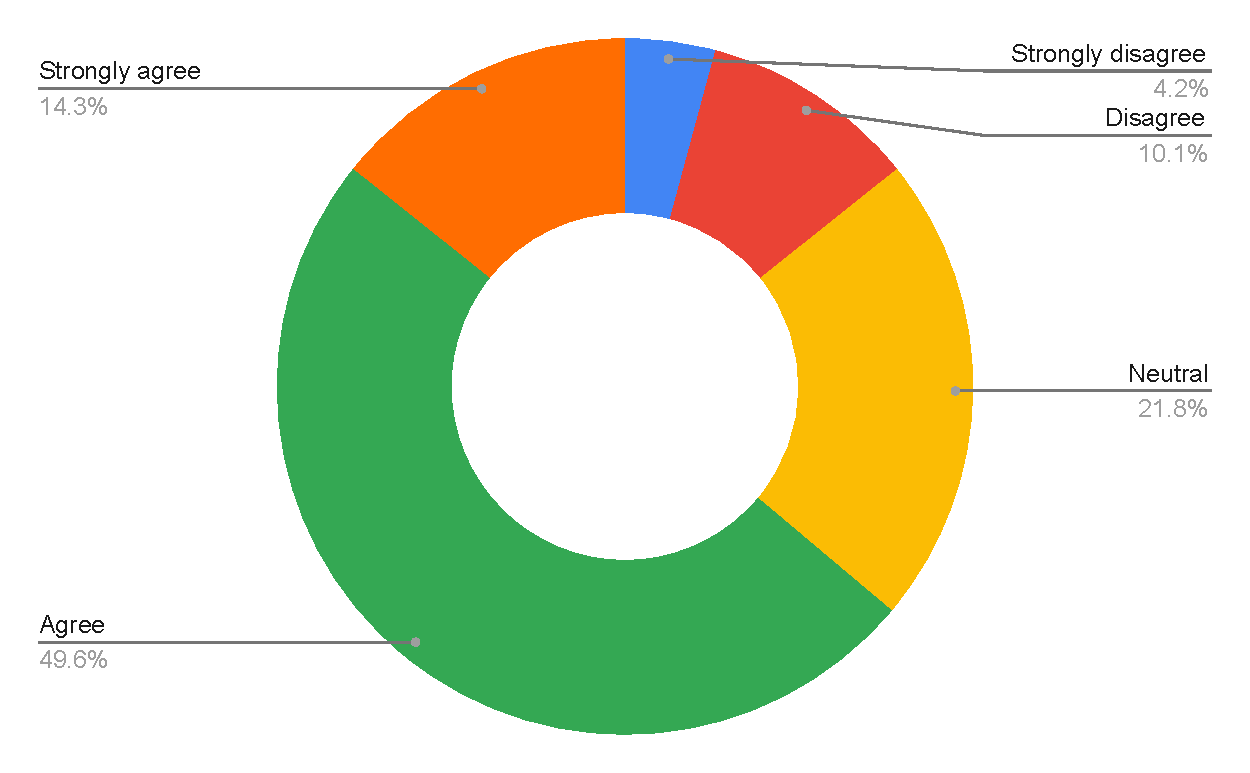
\includegraphics[width=13cm]{thesis/paper/images/p1_q16.pdf}
  \textbf{Question:} I would rather pay a small fee than paying with my data
\end{figure}


\newpage
\subsection{Phase 2 Results}

As mentioned in the previous section, we conducted two separate questionnaire targeting end-users and developers for phase two of our user survey. After removing duplicate submissions and responses with invalid worker ids, we were left with 54 submissions for the end-uses survey, and 14 for the developer survey. Below, we present the response data for answers to each question, with the question text underneath with an indication for which survey the question is from. For both surveys, we include age, country and gender data. For the developer survey, we additionally include years of experience as well.


\begin{figure}[H]
  \centering
  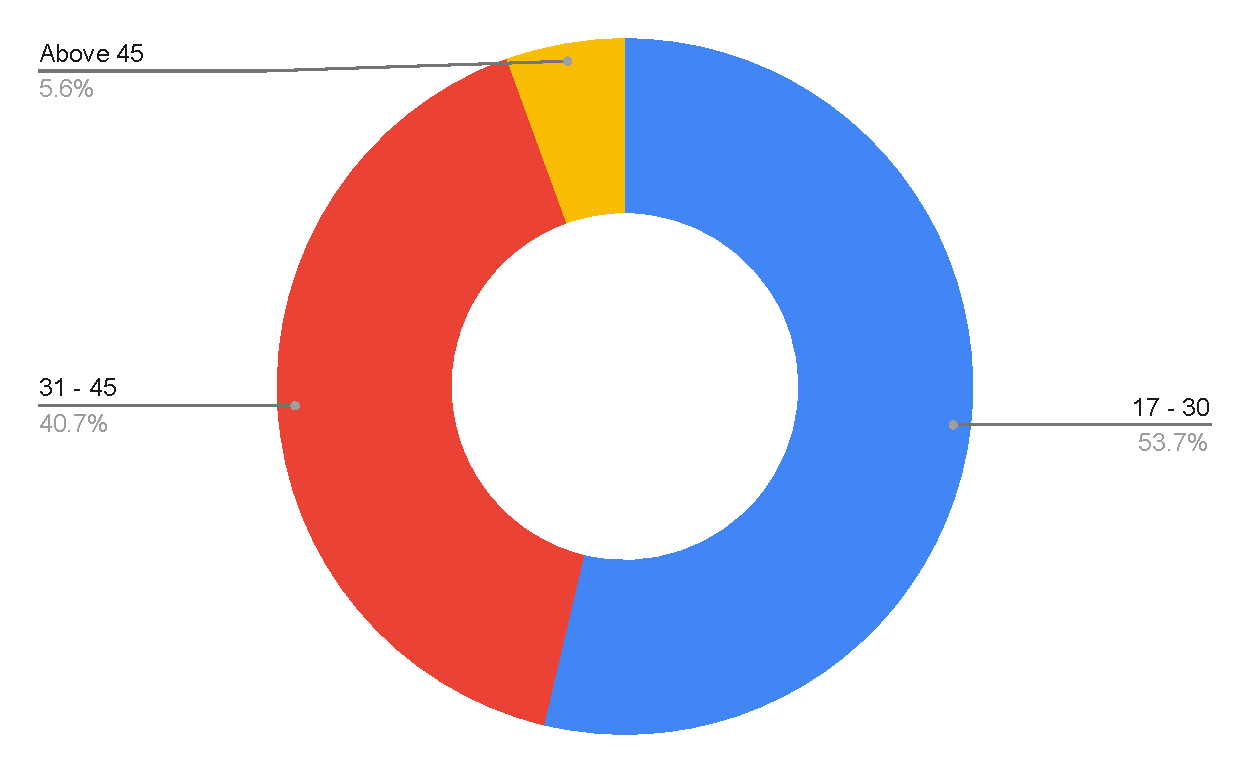
\includegraphics[width=13cm]{thesis/paper/images/p2u_age.pdf}
  \textbf{Age distribution (End-user survey)}
\end{figure}


\begin{figure}[H]
  \centering
  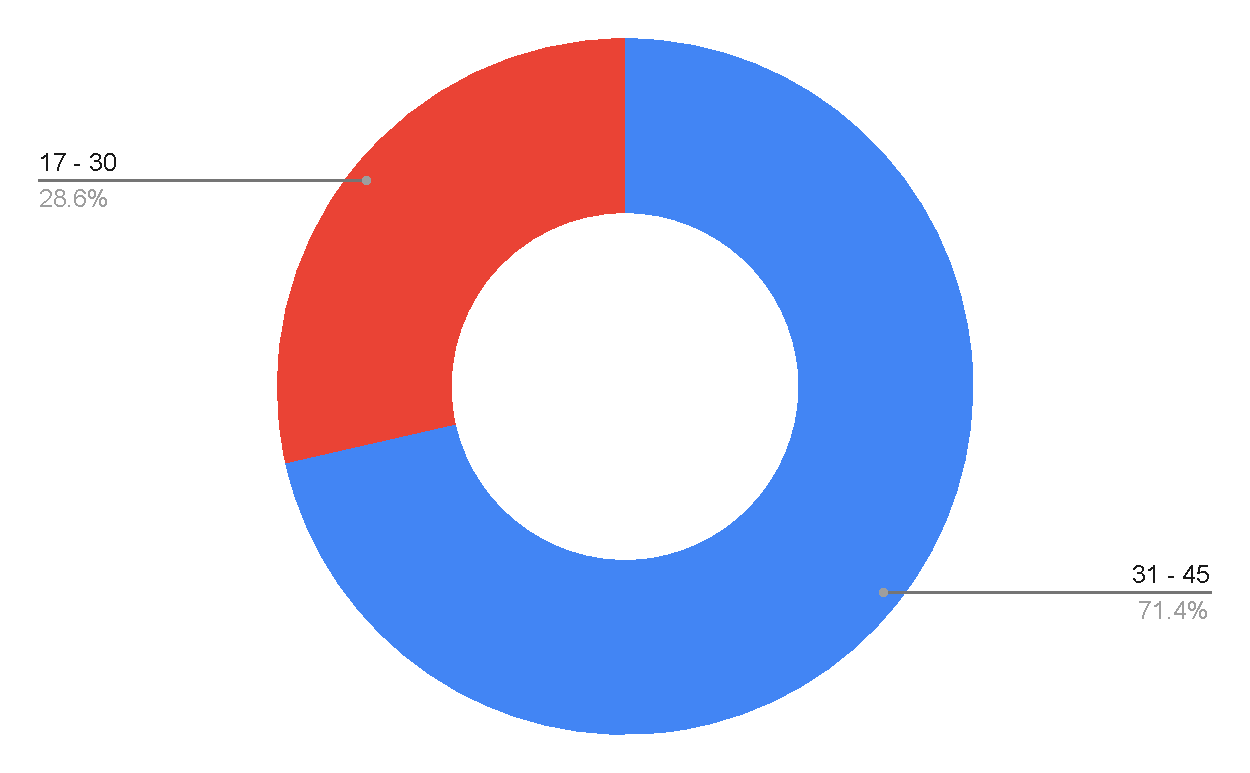
\includegraphics[width=13cm]{thesis/paper/images/p2d_age.pdf}
  \textbf{Age distribution (Developer survey)}
\end{figure}

\begin{figure}[H]
  \centering
  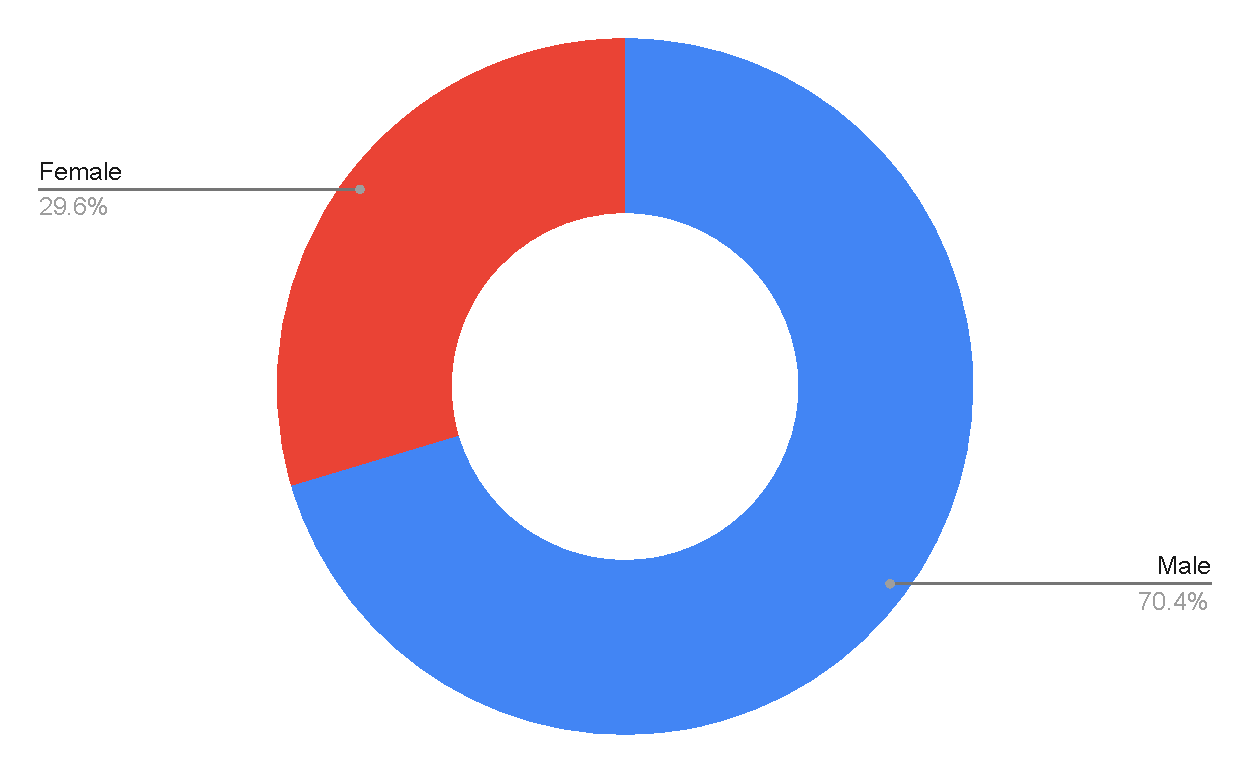
\includegraphics[width=13cm]{thesis/paper/images/p2u_gender.pdf}
  \textbf{Gender distribution (End-user survey)}
\end{figure}

\begin{figure}[H]
  \centering
  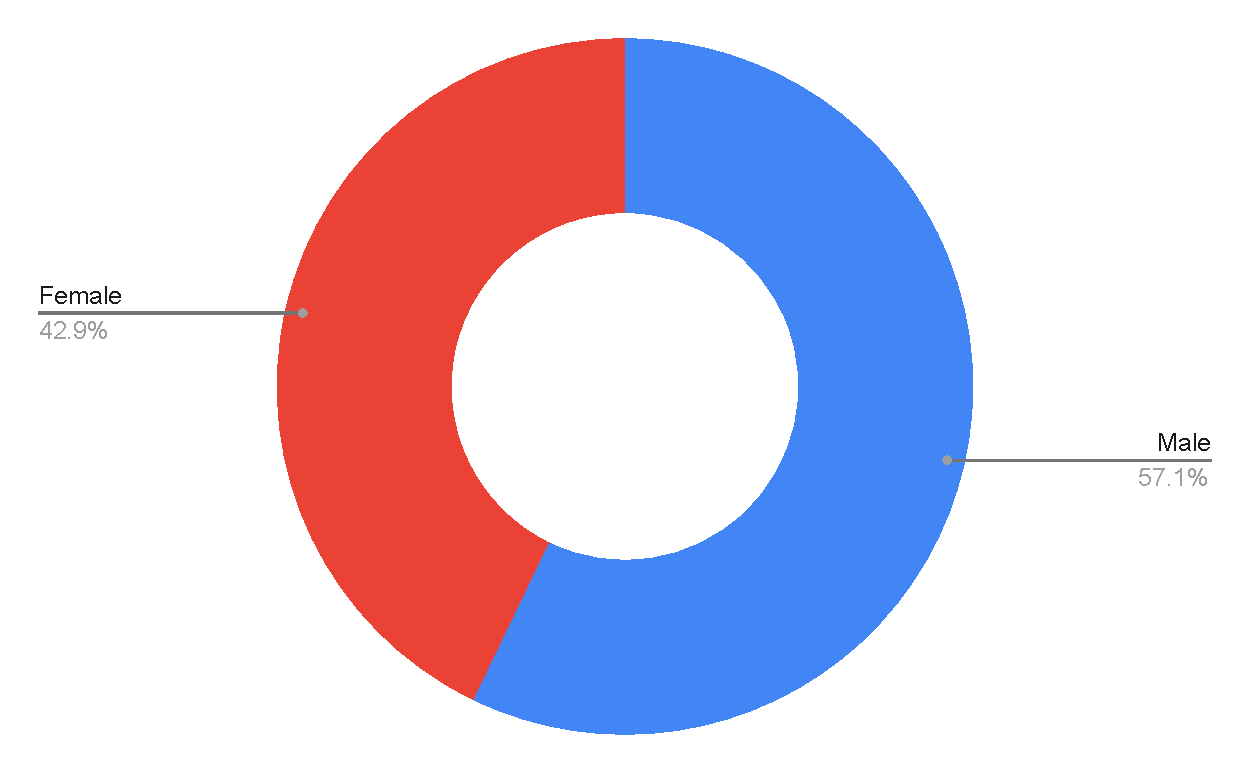
\includegraphics[width=13cm]{thesis/paper/images/p2d_gender.pdf}
  \textbf{Gender distribution (Developer survey)}
\end{figure}

\begin{figure}[H]
  \centering
  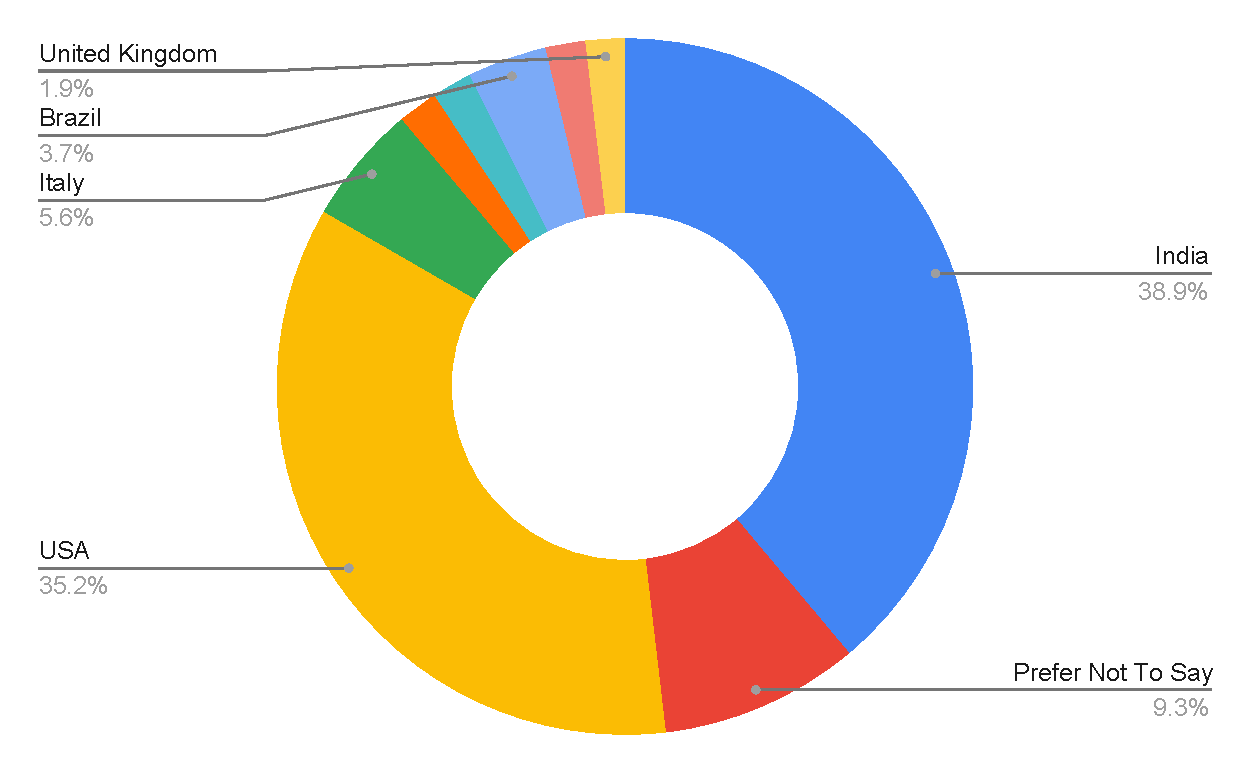
\includegraphics[width=13cm]{thesis/paper/images/p2u_country.pdf}
  \textbf{Country of Origin (End-user survey)}
\end{figure}

\begin{figure}[H]
  \centering
  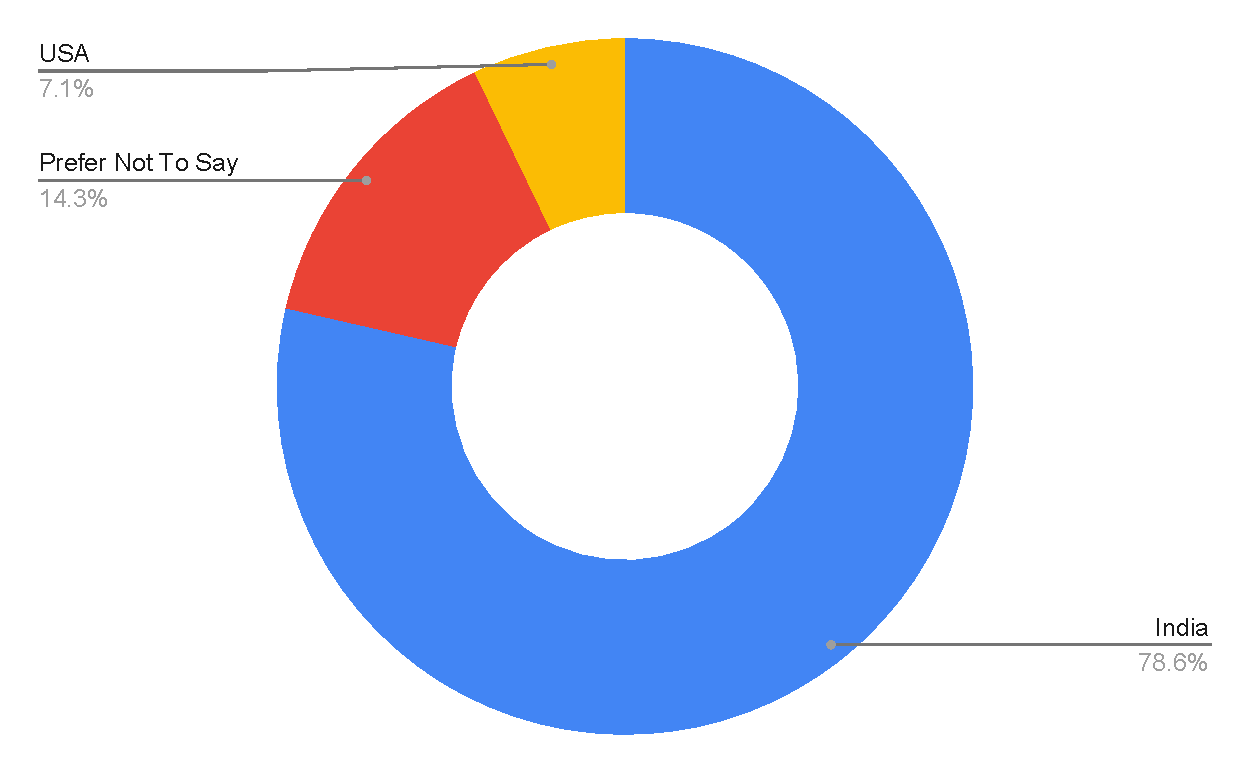
\includegraphics[width=13cm]{thesis/paper/images/p2d_country.pdf}
  \textbf{Country of Origin (Developer survey)}
\end{figure}

\begin{figure}[H]
  \centering
  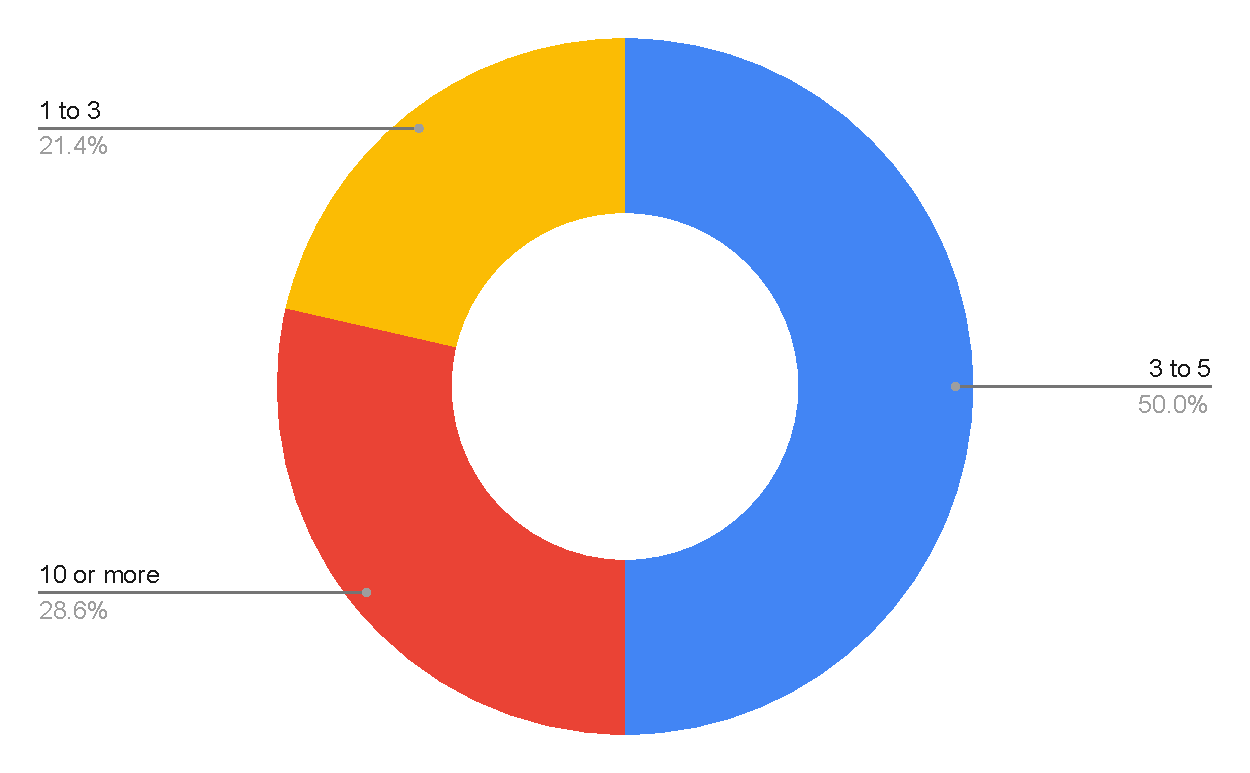
\includegraphics[width=13cm]{thesis/paper/images/p2d_experience.pdf}
  \textbf{Years of Experience (Developer survey)}
\end{figure}

\begin{figure}[H]
  \centering
  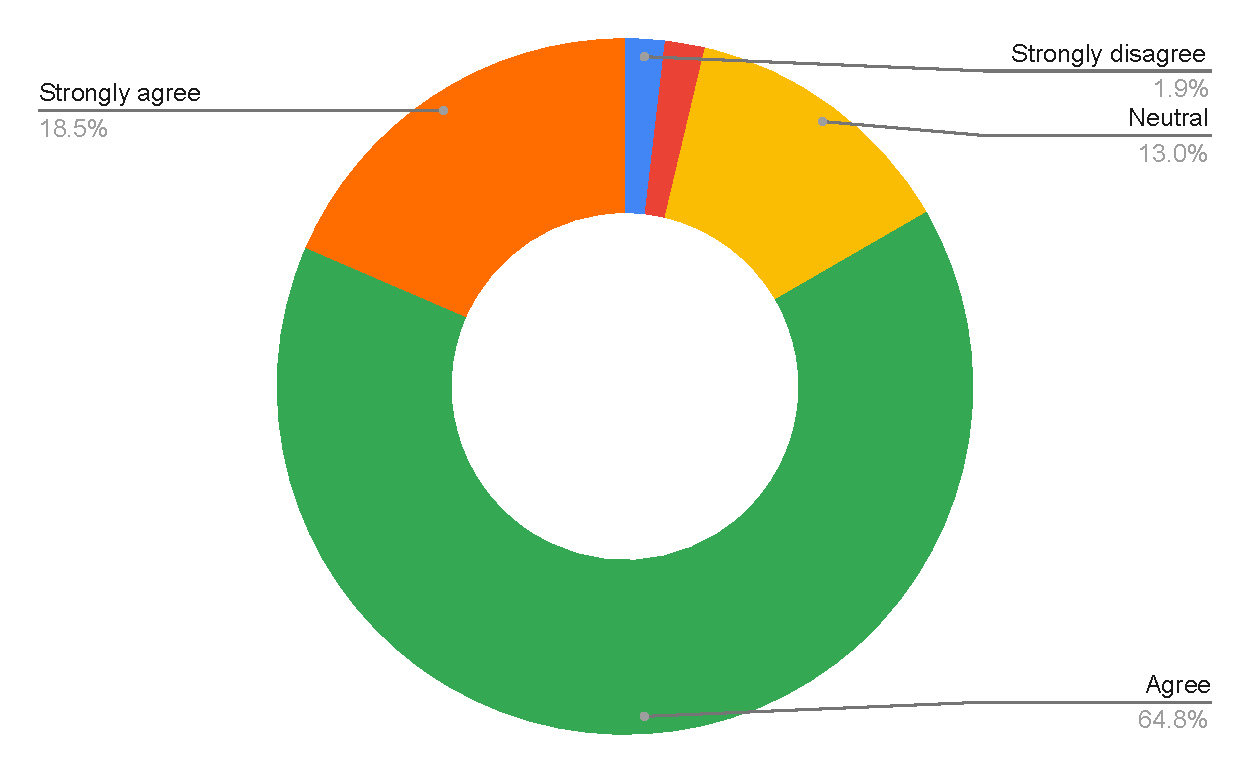
\includegraphics[width=13cm]{thesis/paper/images/p2u_q1.pdf}
  \textbf{Question (End-user survey):} Standardised UI components will improve the consistency across front-end applications
\end{figure}

\begin{figure}[H]
  \centering
  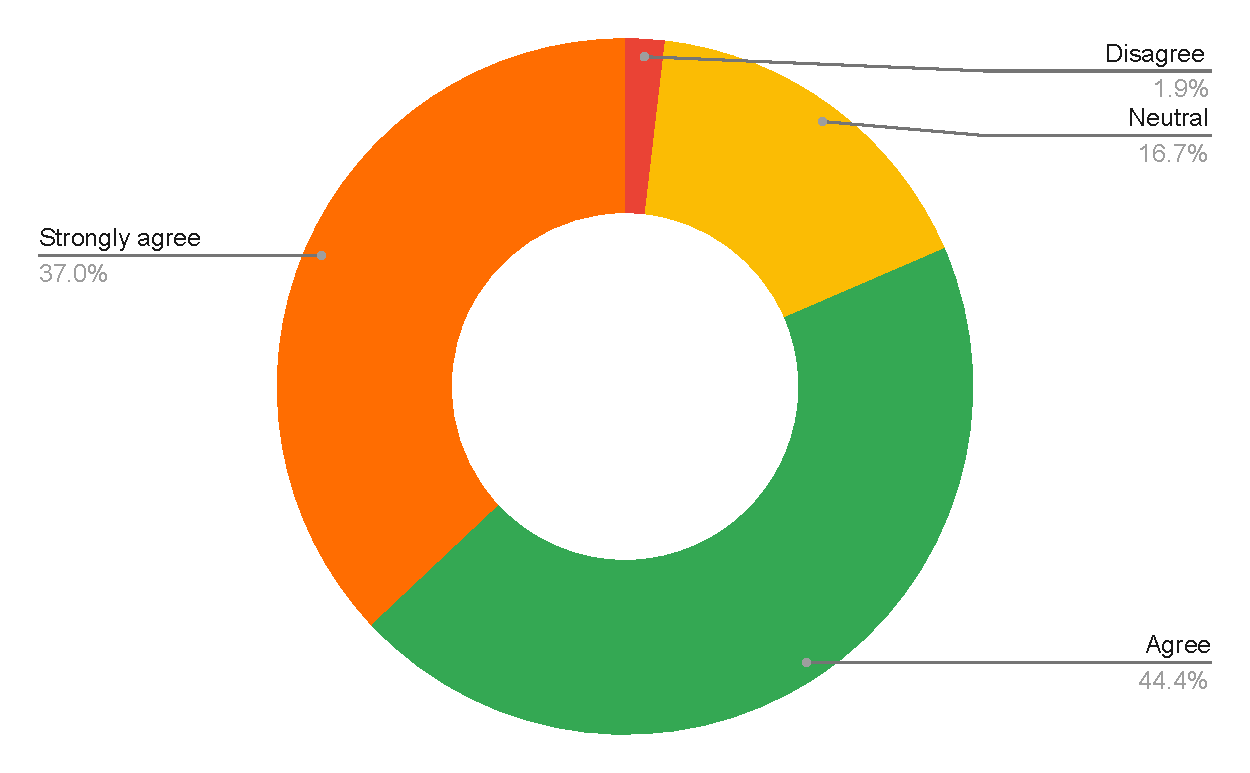
\includegraphics[width=13cm]{thesis/paper/images/p2u_q2.pdf}
  \textbf{Question (End-user survey):} I prefer consistency over variability
\end{figure}

\begin{figure}[H]
  \centering
  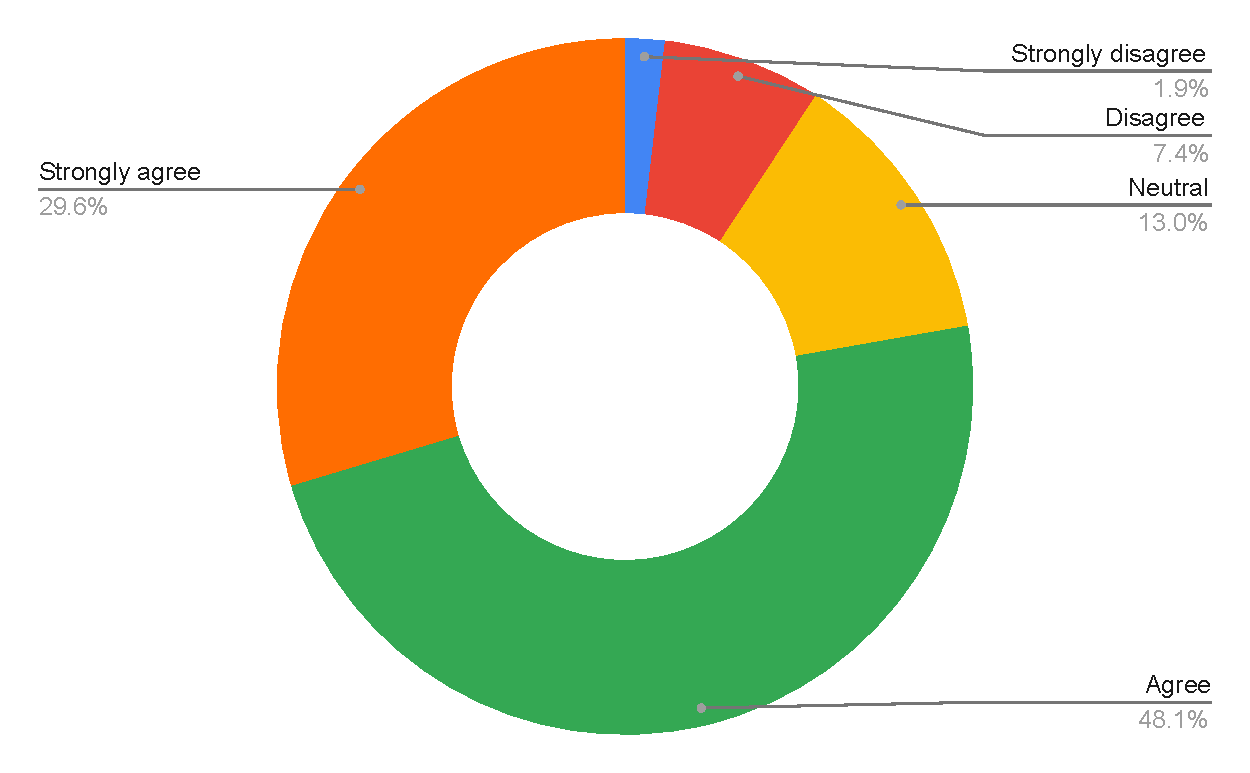
\includegraphics[width=13cm]{thesis/paper/images/p2u_q3.pdf}
  \textbf{Question (End-user survey):} I prefer advertisements to blend in naturally to the look-and-feel of the website instead of sticking out
\end{figure}

\begin{figure}[H]
  \centering
  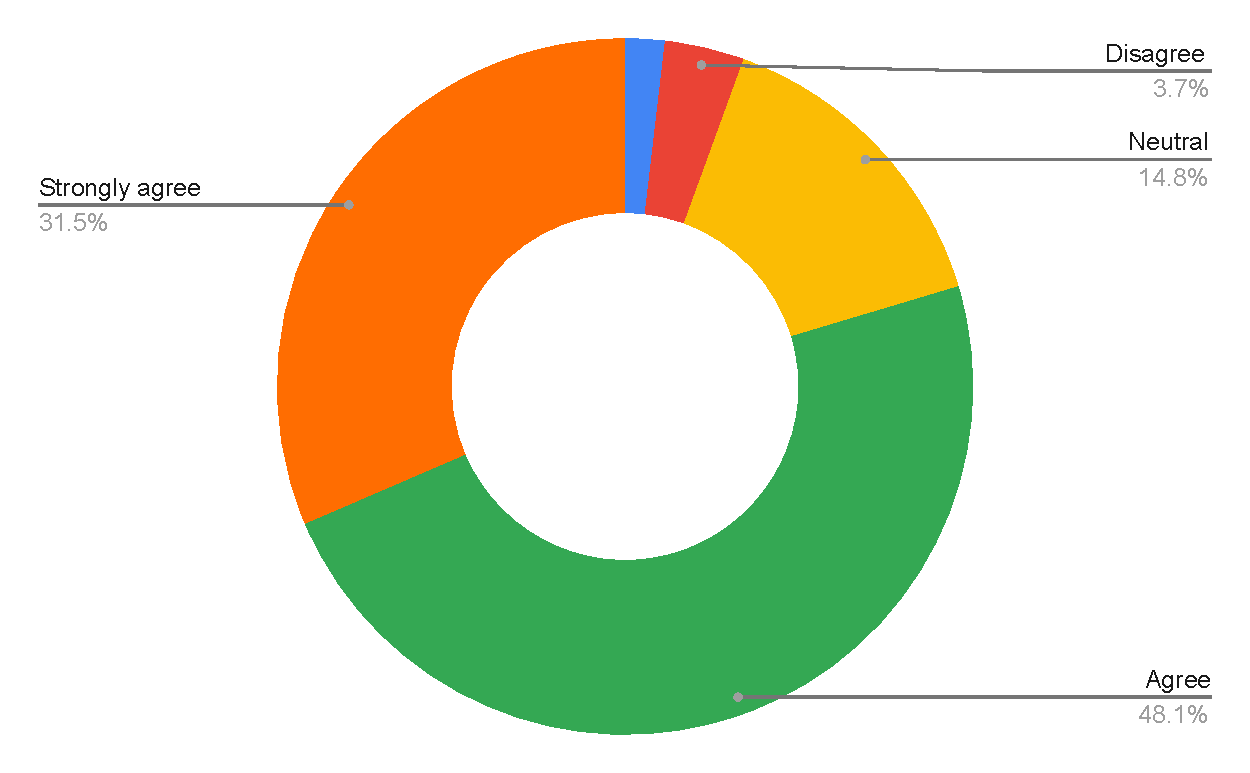
\includegraphics[width=13cm]{thesis/paper/images/p2u_q4.pdf}
  \textbf{Question (End-user survey):} I am okay with seeing non-intrusive and respectful advertisement (with no compromise of privacy), OR paying a small fee in order to support the creator
\end{figure}

\begin{figure}[H]
  \centering
  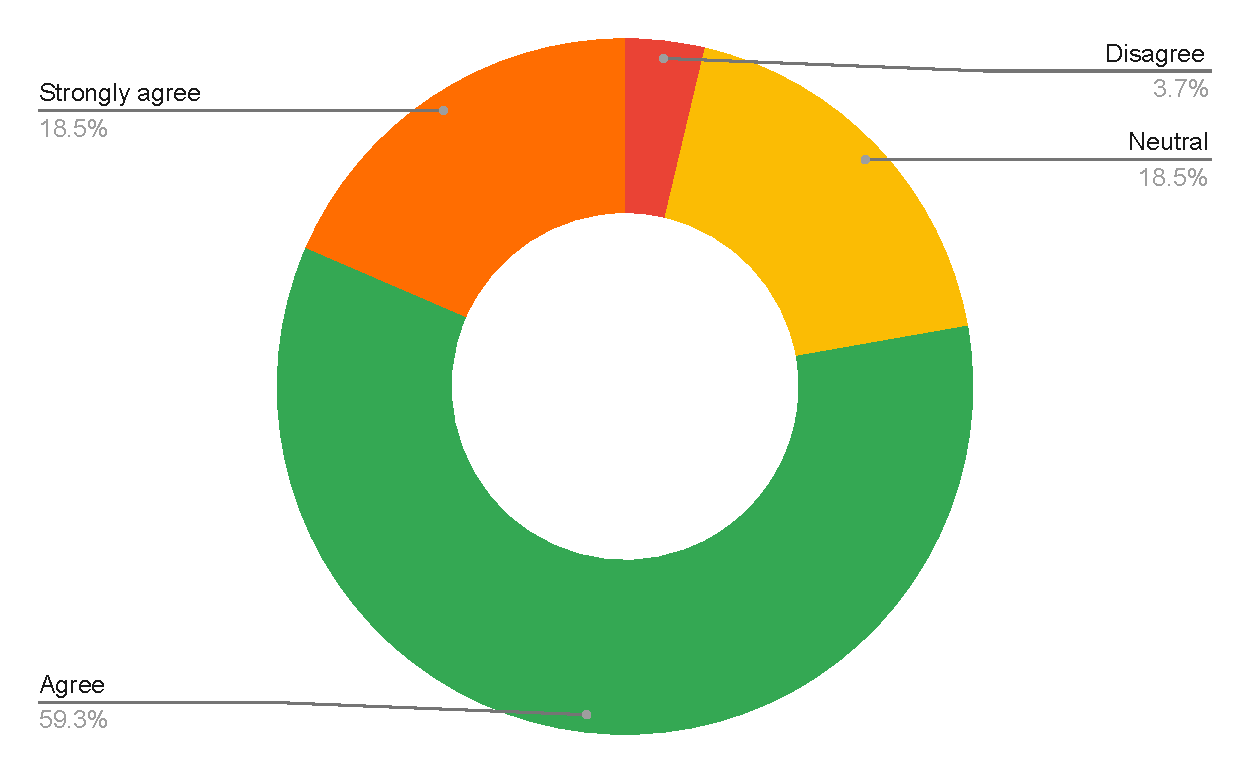
\includegraphics[width=13cm]{thesis/paper/images/p2u_q5.pdf}
  \textbf{Question (End-user survey):} I would benefit from the guaranteed accessibility aspect of Intertext
\end{figure}

\begin{figure}[H]
  \centering
  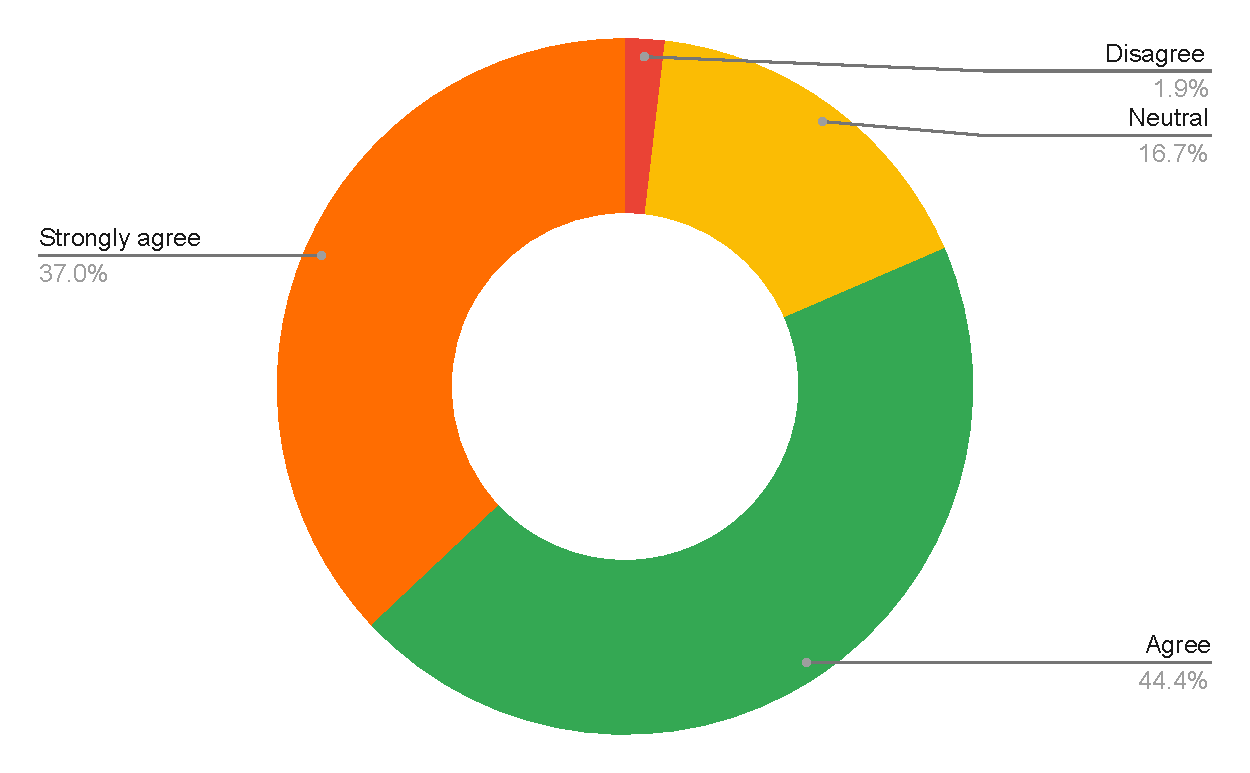
\includegraphics[width=13cm]{thesis/paper/images/p2u_q6.pdf}
  \textbf{Question (End-user survey):} I prefer customisability over variability
\end{figure}

\begin{figure}[H]
  \centering
  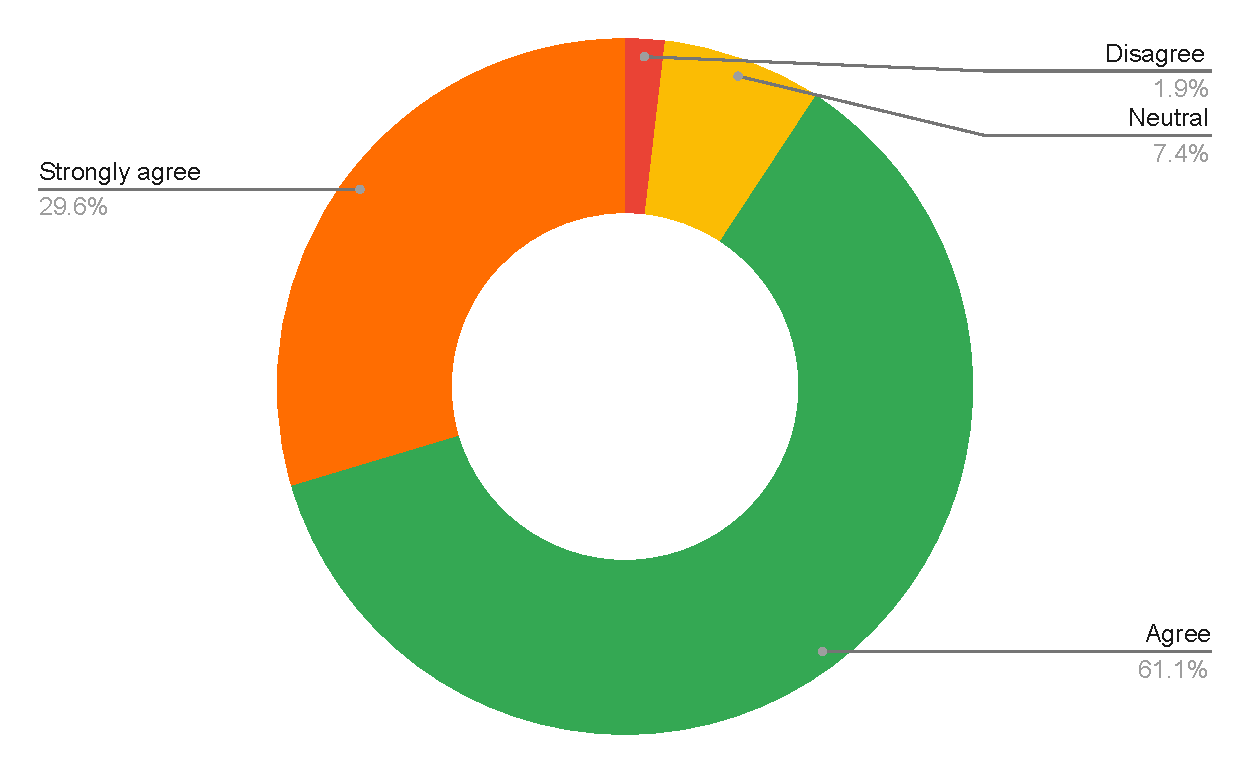
\includegraphics[width=13cm]{thesis/paper/images/p2u_q7.pdf}
  \textbf{Question (End-user survey):} I love that I can create my own theme OR chose a theme I like that applies for all applications
\end{figure}

\begin{figure}[H]
  \centering
  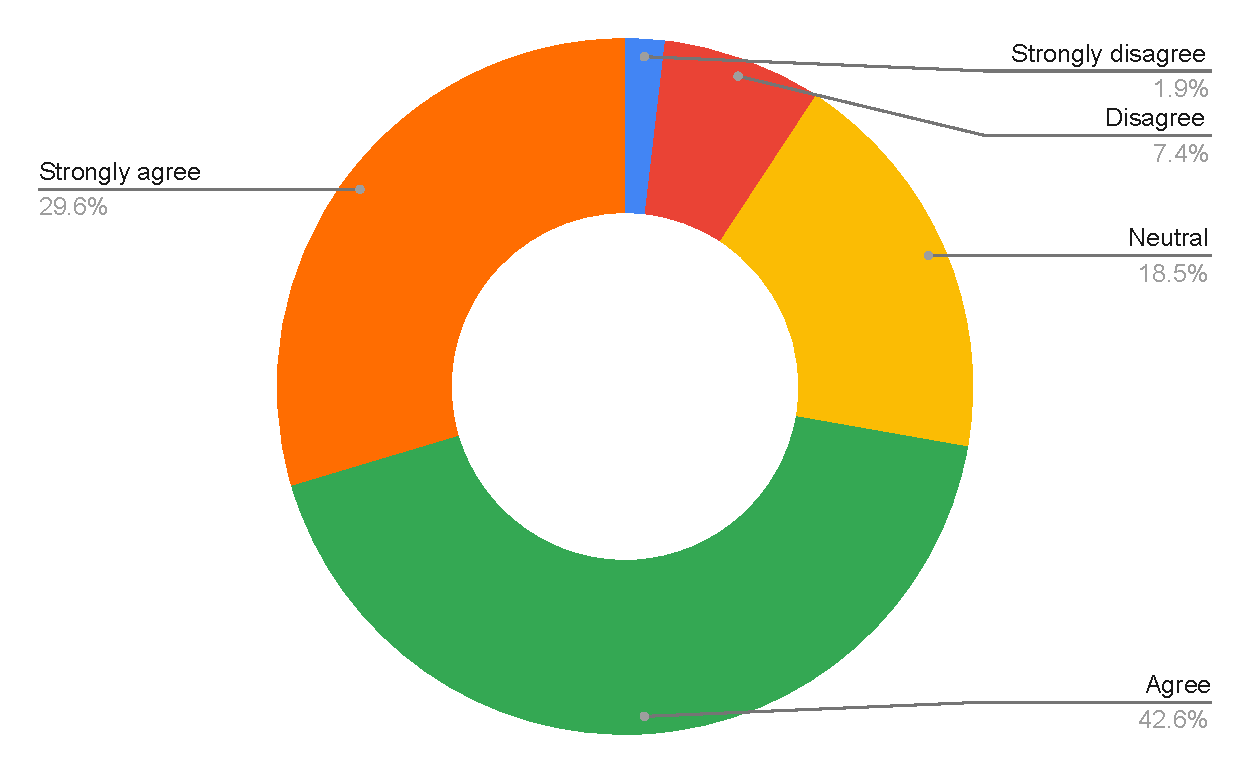
\includegraphics[width=13cm]{thesis/paper/images/p2u_q8.pdf}
  \textbf{Question (End-user survey):} I prefer choosing the look-and-feel I like for all apps, instead of each app having their own look-and-feel
\end{figure}

\begin{figure}[H]
  \centering
  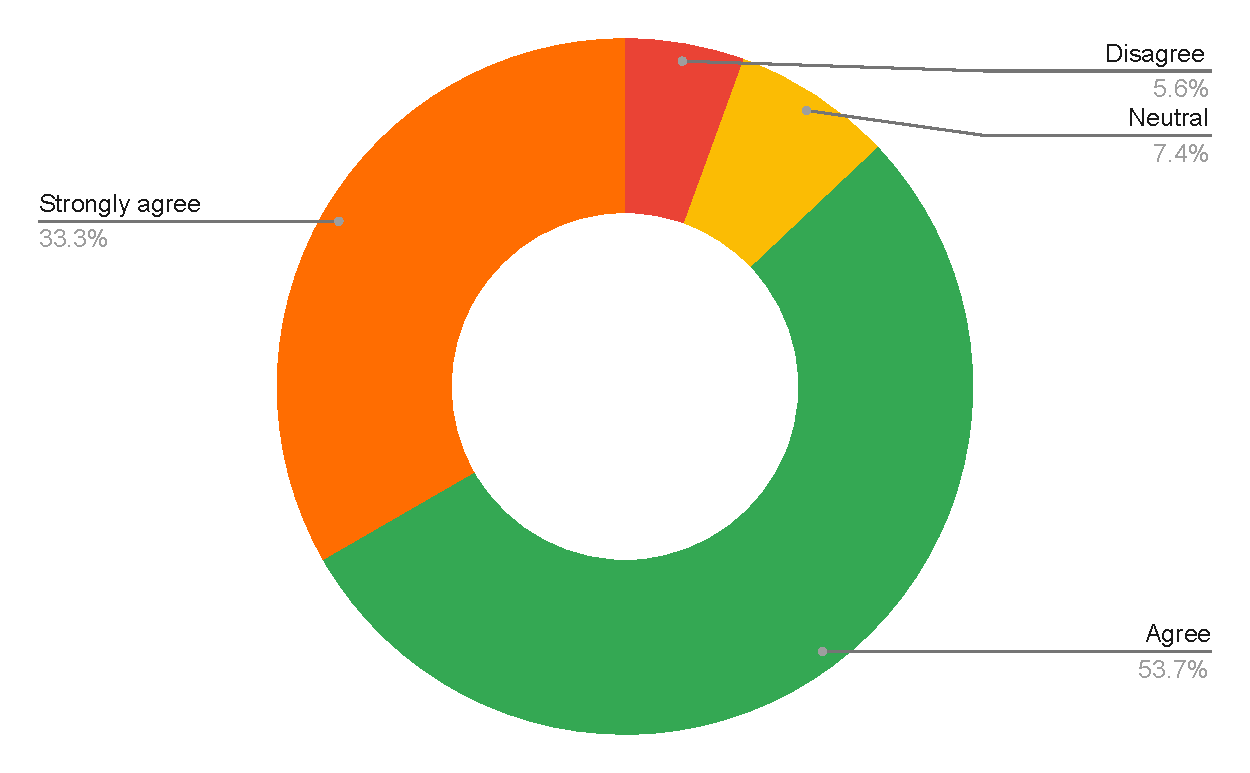
\includegraphics[width=13cm]{thesis/paper/images/p2u_q9.pdf}
  \textbf{Question (End-user survey):} I would be interested in seeing applications running natively on alternative platforms/devices (i.e. other than desktop/mobile - such as wearables, command line interfaces etc.)
\end{figure}

\begin{figure}[H]
  \centering
  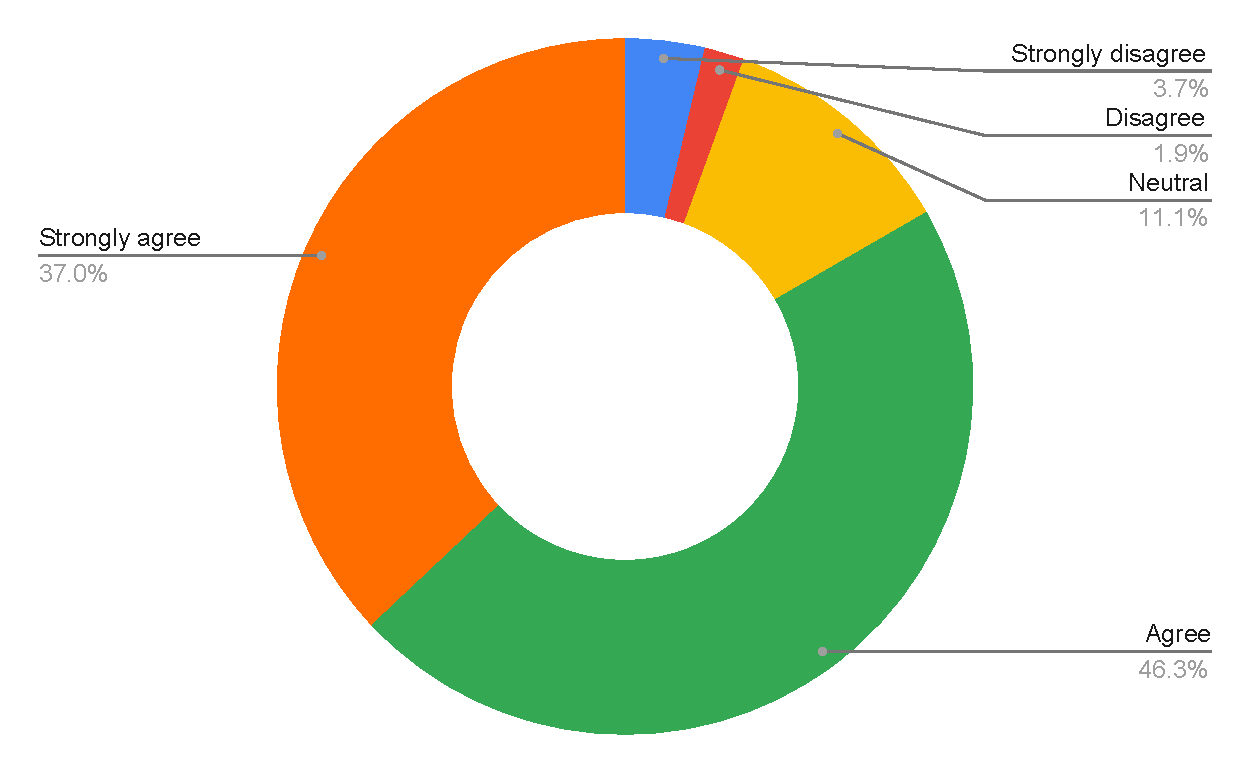
\includegraphics[width=13cm]{thesis/paper/images/p2u_q10.pdf}
  \textbf{Question (End-user survey):} If all devices/platforms/environments supported all applications that I use natively, it would increase the use of my other devices.
\end{figure}

\begin{figure}[H]
  \centering
  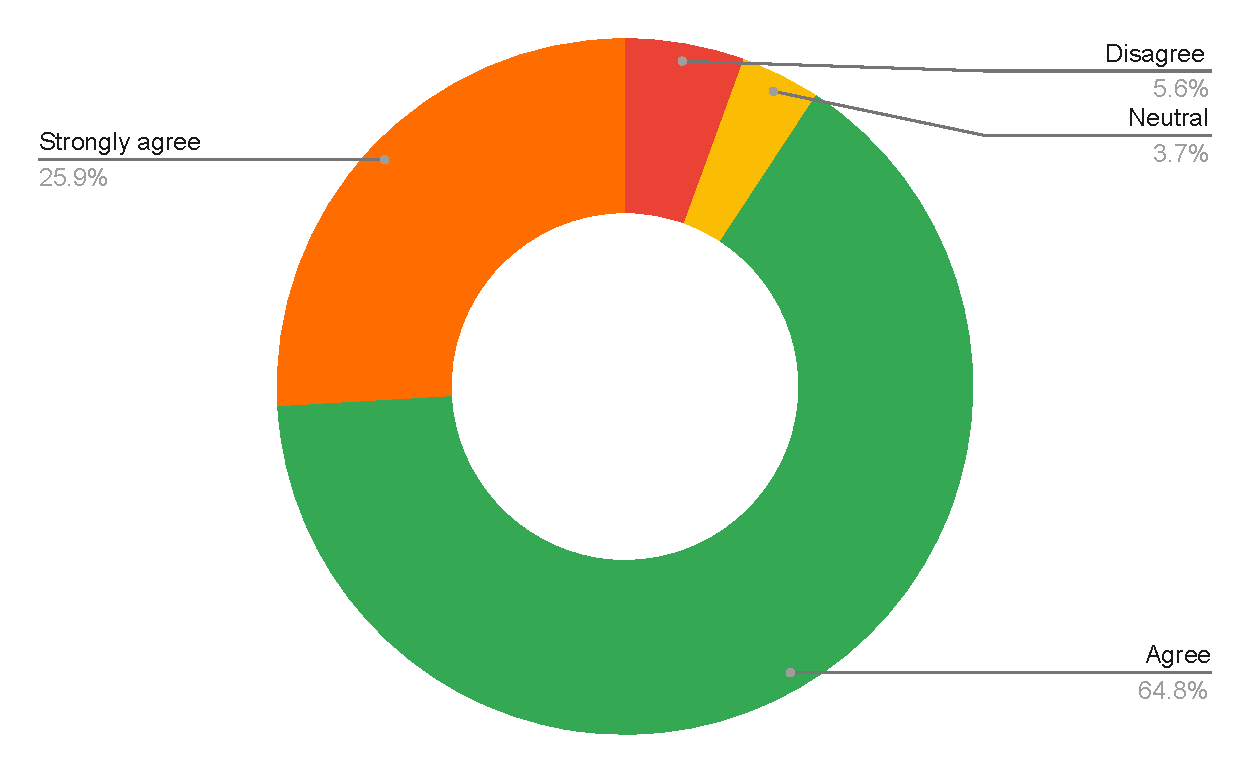
\includegraphics[width=13cm]{thesis/paper/images/p2u_q11.pdf}
  \textbf{Question (End-user survey):} I would prefer guaranteed privacy and security over rich front-end functionality
\end{figure}

\begin{figure}[H]
  \centering
  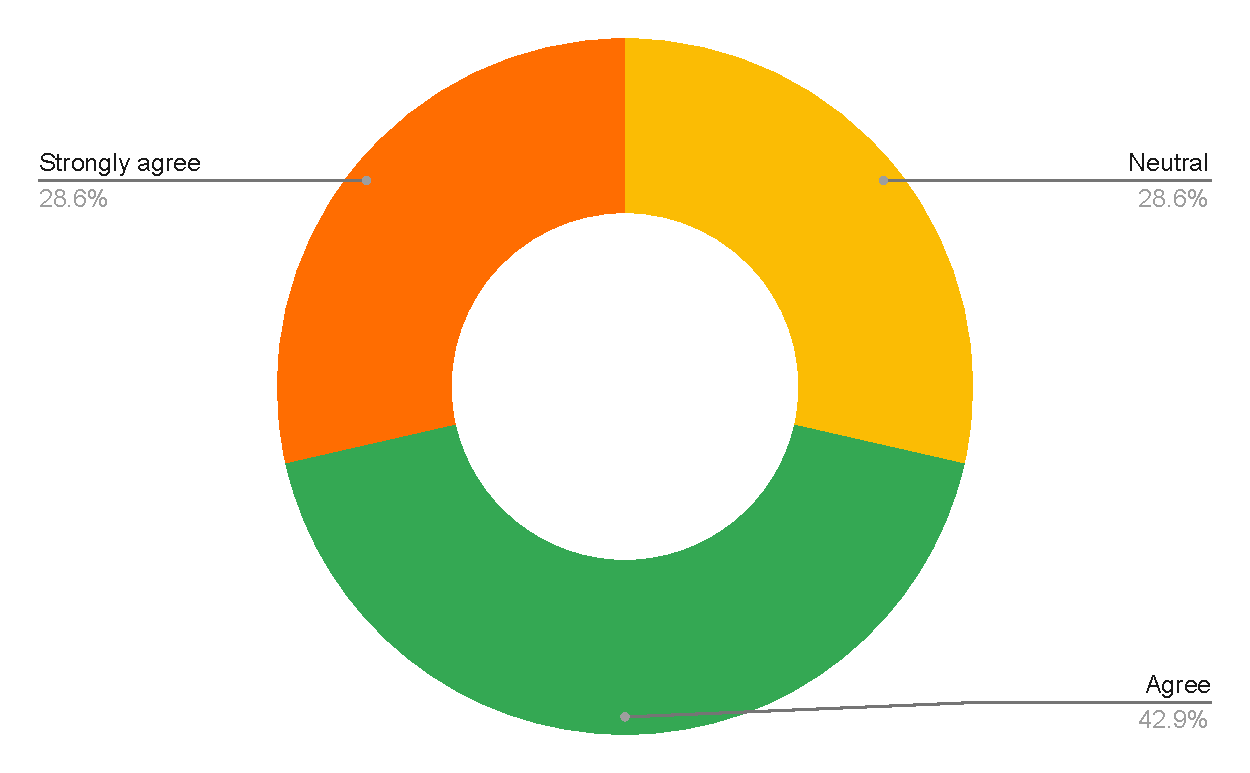
\includegraphics[width=13cm]{thesis/paper/images/p2d_q1.pdf}
  \textbf{Question (Developer survey):} I would prefer using IUIDL over building my own components from scratch with the cost of adding cross-platform support
\end{figure}

\begin{figure}[H]
  \centering
  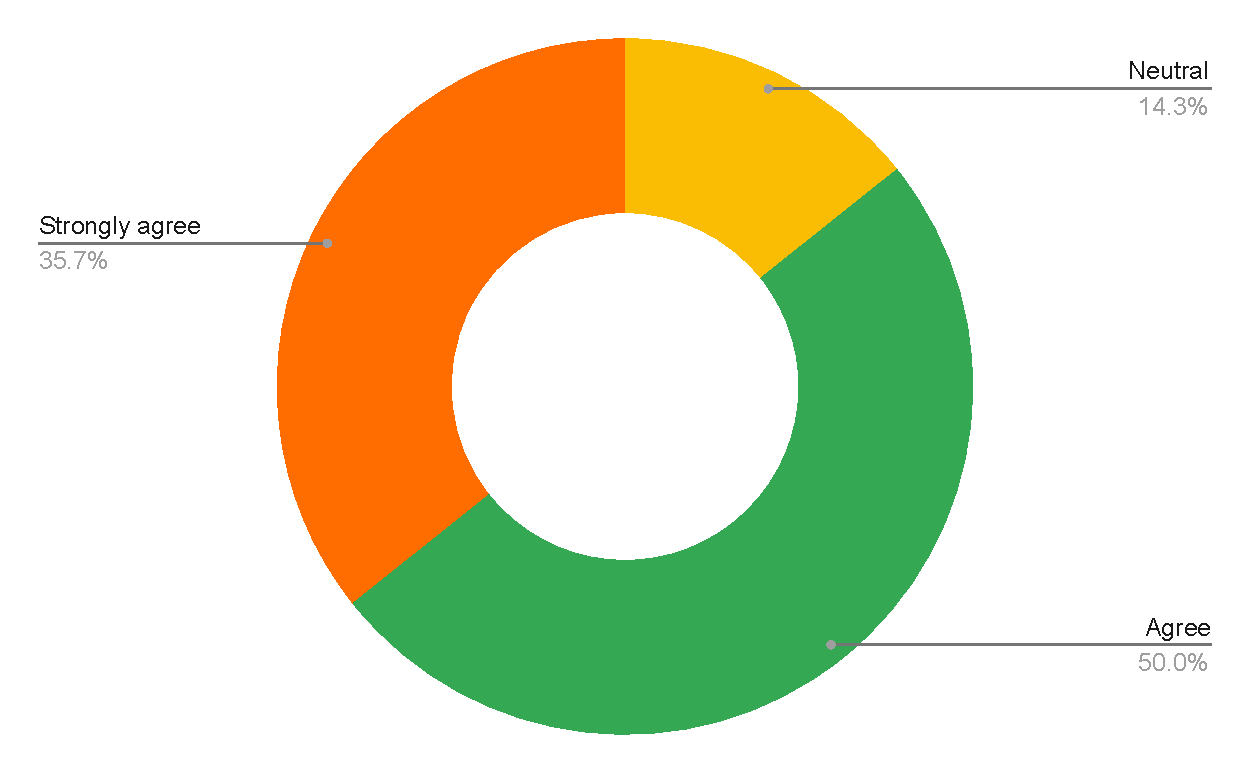
\includegraphics[width=13cm]{thesis/paper/images/p2d_q2.pdf}
  \textbf{Question (Developer survey):} I would prefer using IUIDL over building my own components from scratch with the cost of making them accessible
\end{figure}

\begin{figure}[H]
  \centering
  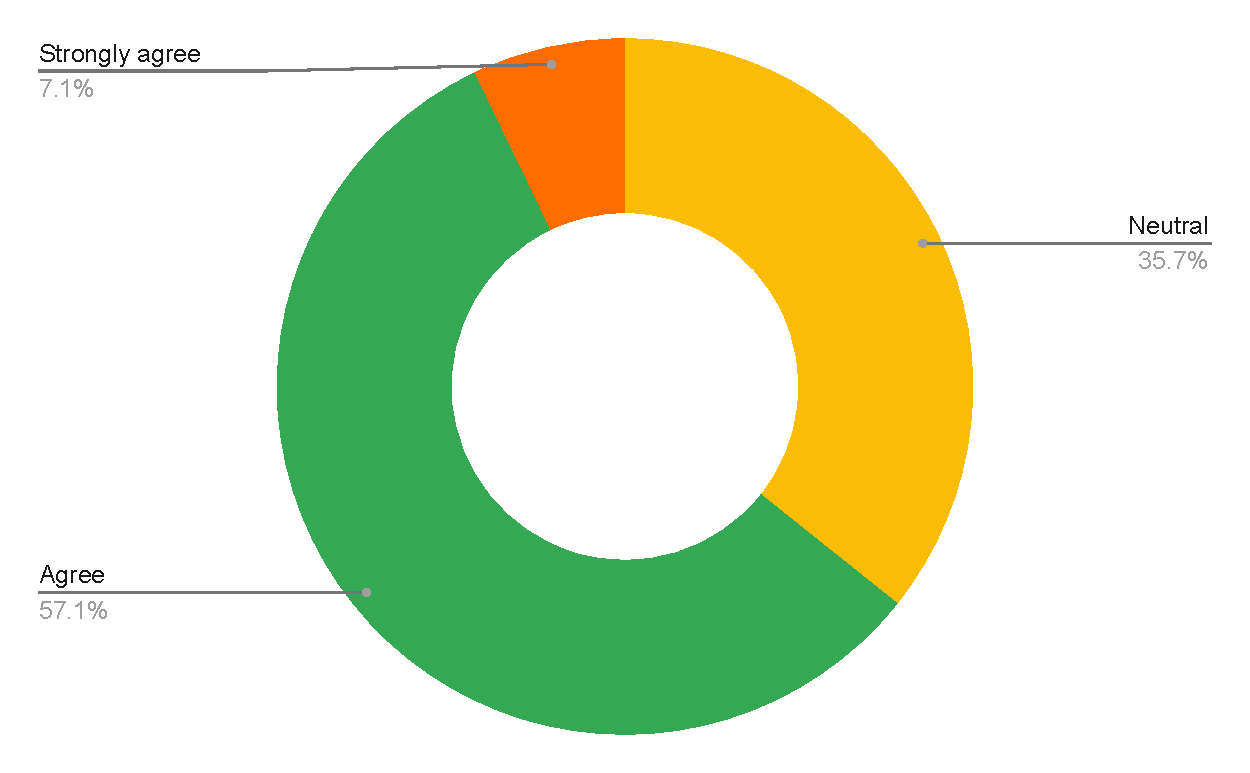
\includegraphics[width=13cm]{thesis/paper/images/p2d_q3.pdf}
  \textbf{Question (Developer survey):} I would prefer using IUIDL over building my own components from scratch with the cost of maintenance
\end{figure}